%%% Local Variables:
%%% mode: latex
%%% TeX-master: t
%%% End:

\chapter{引言}
\label{ch:intro}

\section{光子晶体简介}
\label{sec:intro_PhC}

光与物质之间的作用使得我们所在的世界呈现五光十色的外观。在分子层次上,染料分子通过分子能级来调控光子的行为以显示出颜色;在微观尺度上,则可以通过物质复杂介电常数的结构来进行光的。自然界中常见的结构光现象即是通过后者的机理而形成的\cite{Ball2012NatureS},包括孔雀羽毛、蝴蝶翅膀、蛋白石等著名例子。当物质具有周期性变化的介电常数结构时,会呈出对光调控的特性。这一现象由John与Yablonovitch同时提出\cite{John1987Strong,Yablonovitch1987Inhibited}。由于这一类物质的周期性变化的介电常数结构与晶体类似,将其称为光子晶体(photonic crystal)。物质的晶格使得电子的传播在物质中产生改变,从而形成了电子能带;类似地,电磁波在光子晶体中传播时也具有同样的光子能带结构。当光子晶体的介电常数符合一定条件时,则能够形成独特的光子带隙(photonic band gap, PBG)或称光子禁带。与其匹配频率范围内的电磁波无法在光子晶体中传播。对于光子禁带的调节能够改变光子晶体对电磁波的传播行为,形成复杂的功能材料。

在过去20多年中,光子晶体材料在通讯、物理、化学、生物等较差学科上有着广泛的应用,例如光子陷阱\cite{Baba2008Slow}、高精度信号传输\cite{Adawi2010Optical}、染料激光器\cite{Scofield2011BottomUpa}、光子晶体光纤\cite{Consales2012LabOnFiber,Wang2013FiberOptic}、化学/生物传感器\cite{Zhao2010Photonic}、光子晶体显示\cite{Arsenault2007PhotonicCrystal}等。可以预期,当光子晶体独特的带隙结构与其他学科相互交叉,将会在新材料、传感技术等方向有着巨大的发展潜力。

\subsection{三维光子晶体及其性质}
\label{subsec:3DPhC}

以介电性的周期性重复分类,可以将光子晶体分为一维、二维、三维(1D、2D、3D)光子晶体,如图~\ref{fig:1d2d3d}所示。
\begin{figure}[htbp]
	\centering
	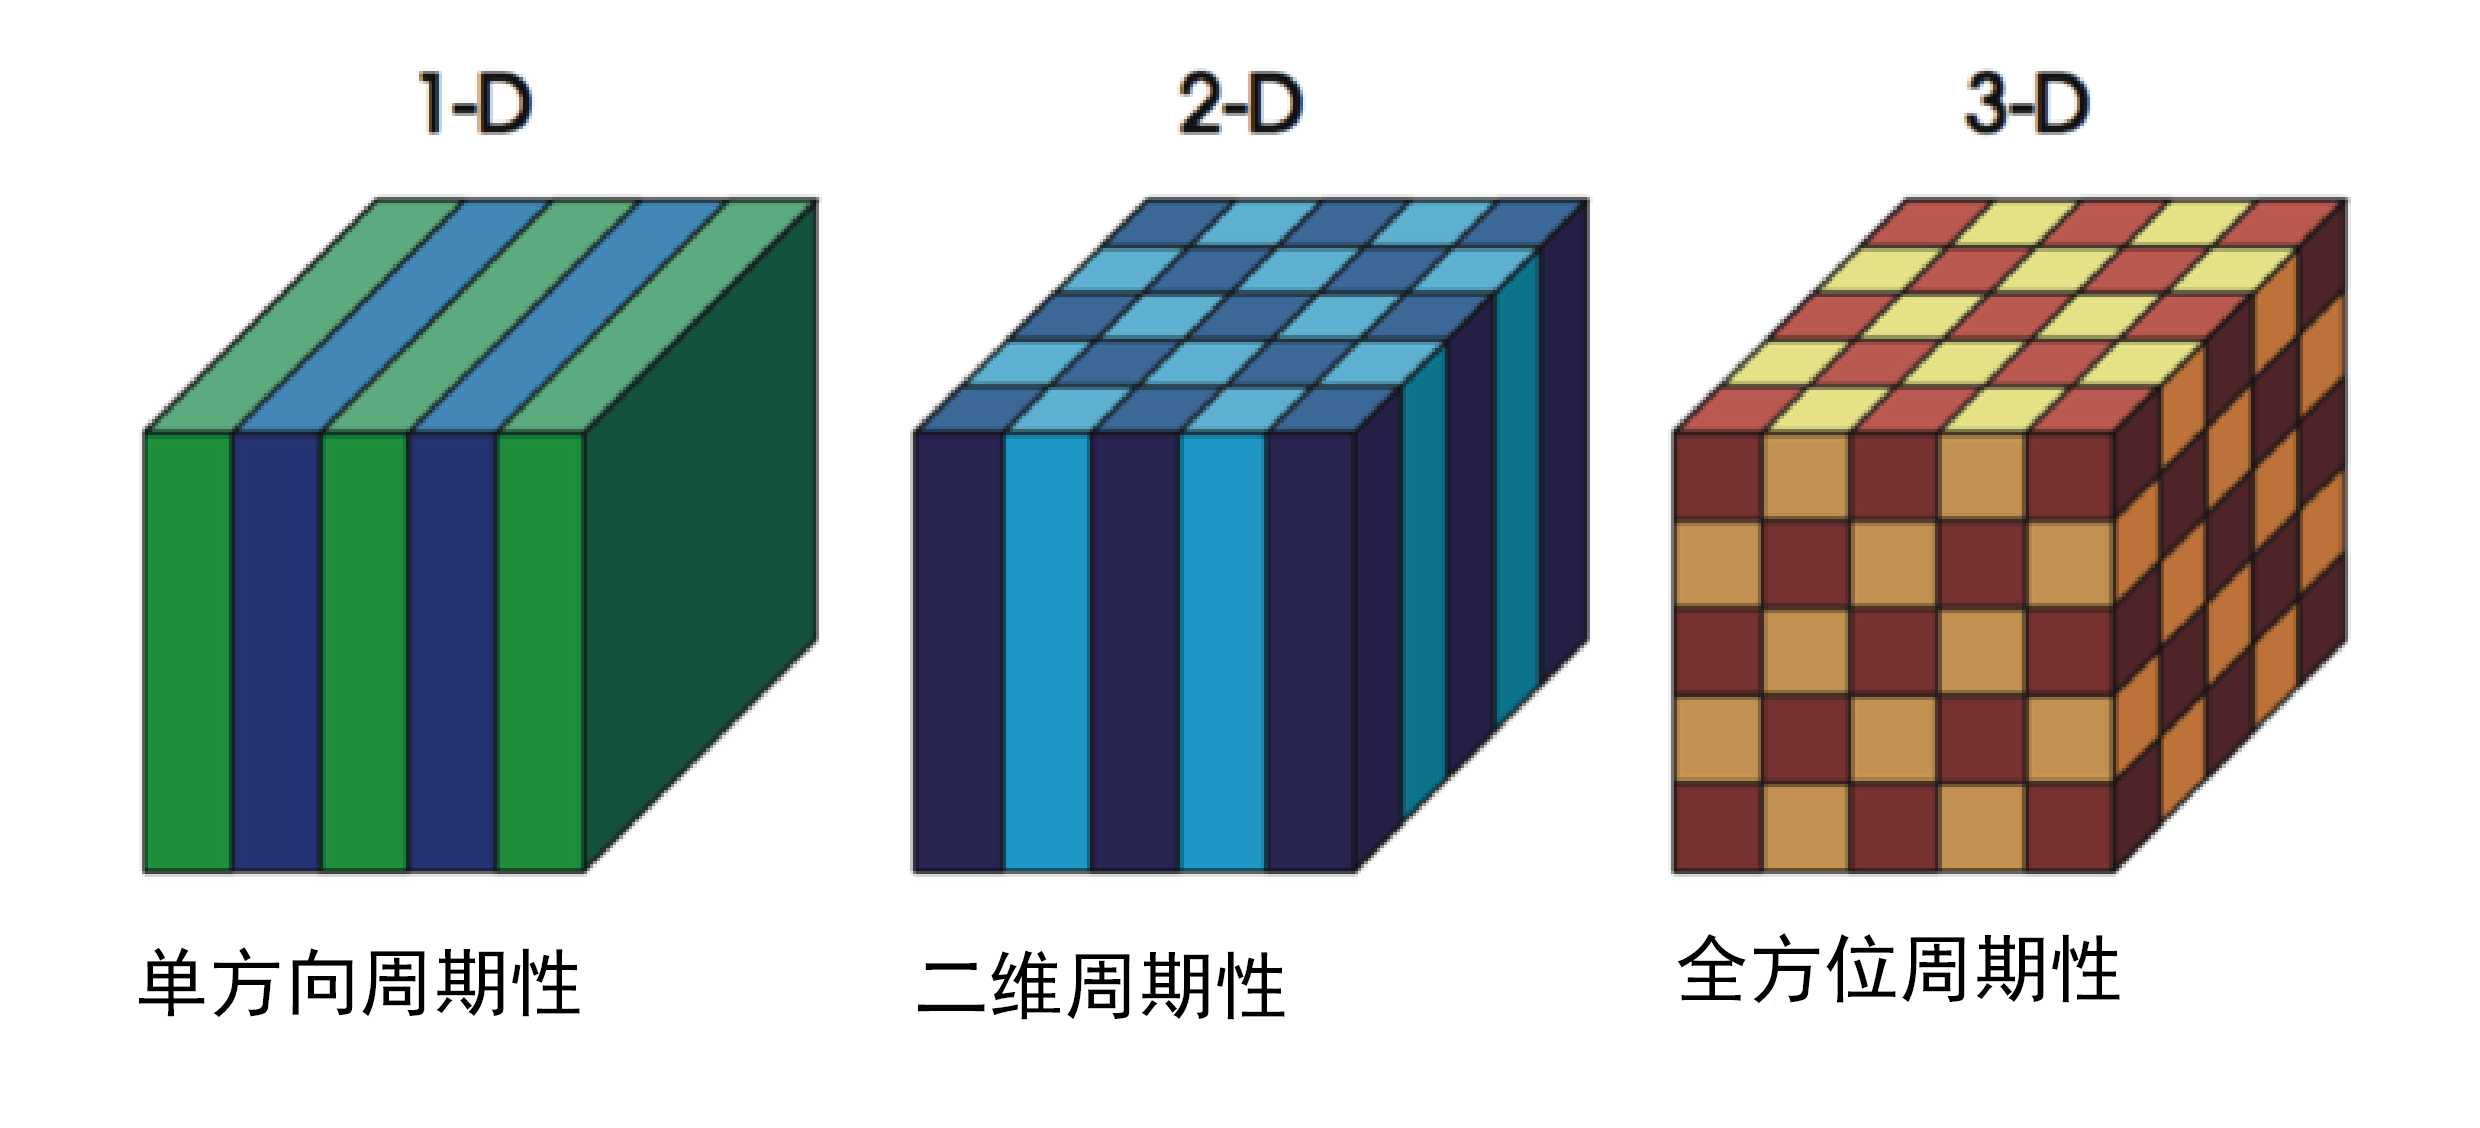
\includegraphics[width=0.85\linewidth]{figures/1d2d3d.png}
	\caption{光子晶体结构示意图}
	\label{fig:1d2d3d}
\end{figure}%
1D的光子晶体结构通常为具有周期性介电常数的多层平面结构,或又称为布拉格反射镜(Bragg mirror),其光子禁带仅存在于周期方向上。同理,当物质在二维或三维空间上均具有周期性结构,则能够具有空间上的光子禁带结构。二维光子晶体具有平面方向上的光子禁带;而三维光子则可能具有全方向上的光子禁带,
或称为完全禁带结构(full band gap)。三维光子晶体的完全禁带结构能达到特定能量的光子在光子晶体中的全方位禁阻,从而完成对光子更为精细的调控。本论文中主要将围绕三维光子晶体结构进行讨论。

与实体晶体相似,3D光子晶体也具有多样性的结构及晶胞参数,但在进行光子带隙的计算上可进行一定简化。
由于光子晶体的整体特性,其光子带隙具有Bragg衍射方程的形式:
\begin{equation}
	\label{eqn:1-bragg}
	m\lambda=2d\sqrt{\sum_{i}n_i^2f_i-sin^2\theta}
\end{equation}
其中,$\lambda$ 为光子禁带对应的中心波长也即衍射光的中心波长,$m$为衍射等级,$n_i$代表各部分的折射率,$f_i$为各部分的体积分数,$\theta$代表入射光的方向。
可以注意到,3D光子晶体的光子禁带是角度依赖的;同时,改变物质的折射率$\theta$、晶格参数$d$均能够引起光子禁带的移动,反映在物质的表观状态上即为其反射光颜色发生偏移。光子晶体的这种性质使其
成为了一种理想的信号自表达平台,即物质的内在性质改变能够直接成为可读取的光信号,而无需其他标记分子
辅助。且这种性质改变能够由多种外界刺激引起,使得光子晶体性质的调控具有
多样性,例如溶剂等引起的折射率改变\cite{Higashiguchi2012SolventResponsive,Wang2011Size}、聚合物膨胀\cite{Fudouzi2003Colloidal}、机械力\cite{Haque2011Rapid,Wang2014Robust}、电场作用力\cite{Arsenault2007PhotonicCrystal,Han2014Structural} 、磁场作用力\cite{Ge2009Magnetochromatic,Caicedo2011Magnetophotonic}等。


除了光子禁带结构以外,三维光子的周期性结构也具有其独特的性质。
最为常见的三维光子晶体结构由胶体颗粒堆积而成,称为胶体晶体(colloidal crystal)。
当胶体晶体堆积结构为紧密堆积时,与自然界中的蛋白石(opal)结构相似。
此类光子晶体中,胶体颗粒占大部分体积,空气占较少一部分。
而与此相对的,胶体晶体可以通过模板复制等方法来制备其互补结构,称为反
蛋白石结构(inverse opal)。两者之间的关系可见于图~\ref{fig:opal_inv_opal}。
\begin{figure}[htbp]
	\centering
	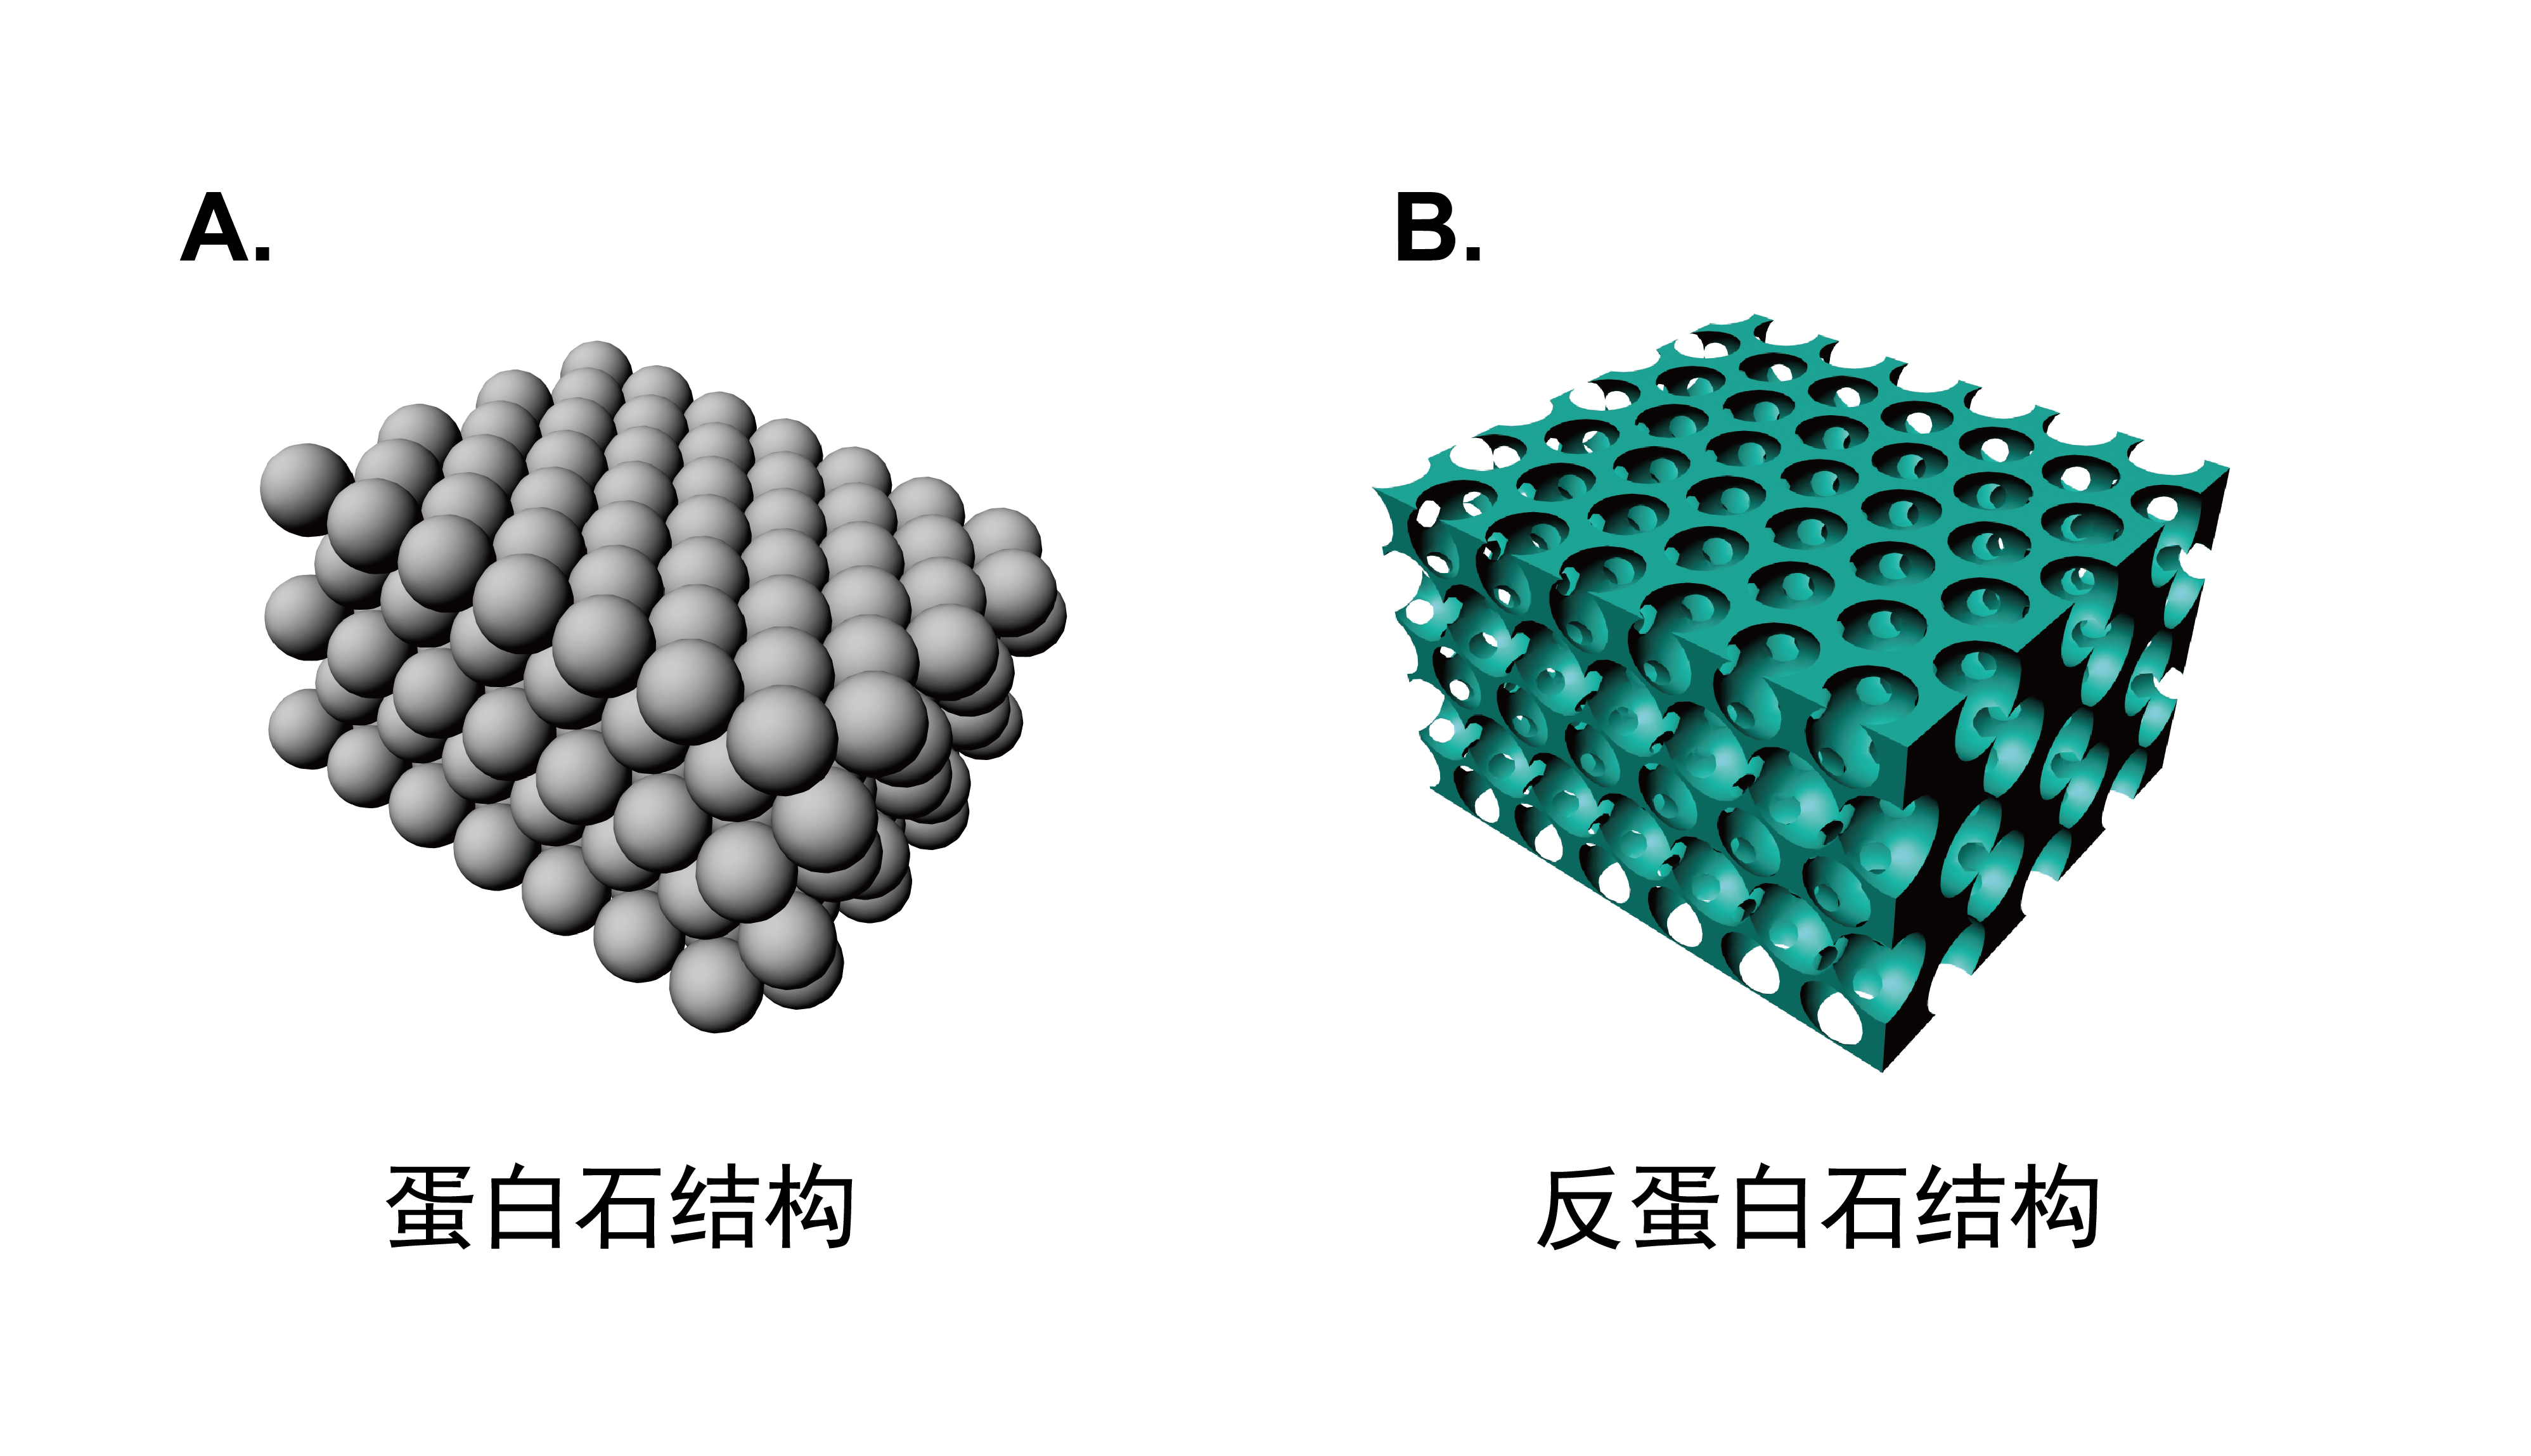
\includegraphics[width=0.75\linewidth]{figures/opalvsinv.png}
	\caption{蛋白石与反蛋白石光子晶体结构示意图}
	\label{fig:opal_inv_opal}
\end{figure}
蛋白石结构与反蛋白石结构的三维光子均具有光子禁带结构,但在功能化方面,
反蛋白石结构更具优势。一方面,由胶体颗粒堆积形成的蛋白石胶体晶体的机械强度较差,而反蛋白石结构由于其整体性而具有较高的稳定性及可操作性;其次,蛋白石的组成受限于胶体颗粒的材料,而反蛋白石光子晶体的组成材料跨度很广泛,可以为
聚合物、无机氧化物甚至单质材料\cite{Meseguer2002Synthesis,Stein2013Design}等;此外,反蛋白石光子晶体材料不同于蛋白石的另一重要特征在于其内部连续贯通的孔道的结构及较大
的比表面积,使其作为一种微孔材料而在电池电极\cite{Kang2012Inverse,Zhou2014Photoelectrodes}、生物基质\cite{Lu2014Hybrid,Kim2014CellFriendly}、膜分离材料\cite{Kim2014Inverse,Kang2014LiquidImpermeable}等方面具有重要的应用。

\subsection{三维光子晶体的制备方法}
\label{subsec:3Dpreparation}
三维光子晶体的制备方法多种多样,其主要制备机理可以分为机械加工、刻蚀加工、
及自组装驱动等。本节中将主要介绍不同方法在光子晶体制备中的应用及其局限性。

(1)机械加工法

机械加工法主要多见于早期光子晶体的制备报道中,比较著名的例子是1991年Yablonovitch等通过逐级钻孔方法制备的Yablonite光子晶体\cite{Yablonovitch1991Photonic}。
Yablonite光子晶体包含面心立方(fcc)结构,同时也是第一个被报道制备的具有完全光子禁带的光子晶体材料(图~\ref{fig:yablonite})。
\begin{figure}[htbp]
	\centering
	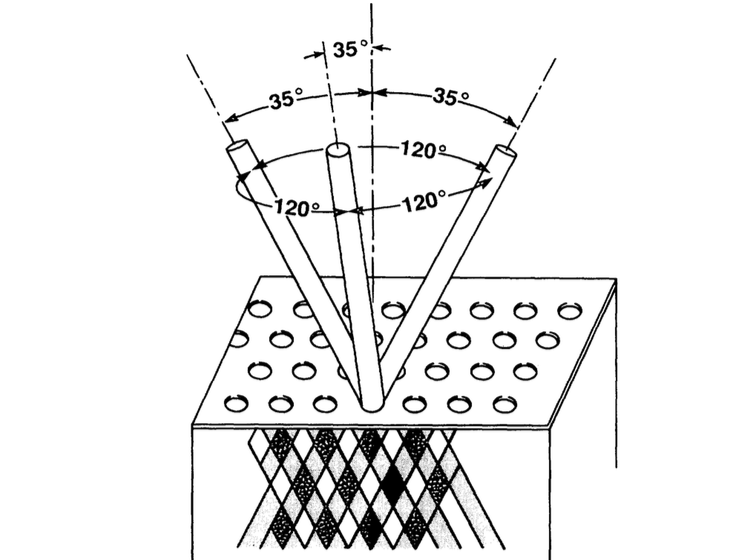
\includegraphics[width=0.6\linewidth]{figures/yablonite.png}
	\caption{Yablonite光子晶体的制备方法\cite{Yablonovitch1991Photonic}}
	\label{fig:yablonite}
\end{figure}
然而受限于机械加工的精度限制,这种加工方法只能应用于微波波段的光子晶体研究。而公式\ref{eqn:1-bragg}表明在可见光波段的光子晶体其周期性结构的尺寸为亚微米尺度,因此需要更为精细的纳米加工方法来制备可见光及近红外波段上的光子晶体材料。

(2)物理刻蚀法

物理刻蚀法在制备三维光子晶体,特别是复杂结构的光子晶体上具有广泛的应用。
电子束刻蚀、反应离子束刻蚀等技术在微电子加工方法已经发展相当完善,在此基础上衍生了一系列通过逐层刻蚀方法制备三维光子晶体的方法。通过该方法制备的三维光子晶体结构
非常多样,包括六方反蛋白石结构\cite{Johnson2000ThreeDimensionally}、木堆结构\cite{Lin1998ThreeDimensional,Noda2000Full}、金刚石结构\cite{Qi2004ThreeDimensional}等。逐层电子束刻蚀的另一个特点是对结构的局部缺陷的控制,能够实现在特定位置形成缺陷,
以制备高品质因素的三维光子晶体材料\cite{Blanco2000LargeScale,Juarez2004Selective}。然而电子束或反应离子束刻蚀等方法也存在着其显著的局限性。适用于电子束刻蚀的材料大多为无机材料,包括半导体与金属等,在高分子上的应用有限;其次,逐层刻蚀
非常耗时,工序复杂,在制备大规模的光子晶体上限制较多。利用逐层交替(layer-by-layer,LbL)方法与电子束刻蚀相结合能够一定程度上降低电子束刻蚀的复杂度,
以制备较大的三维光子晶体\cite{Aoki2002ThreeDimensional,Aoki2003Microassembly}。

利用电子束或反应离子束进行刻蚀通常需要大量的掩膜与去除步骤,而利用激光刻蚀能
够达到无掩膜刻蚀的目的。一种较为直接的方法为使用双光子替代电子进行刻蚀,例如
利用该方法制备的木堆型光子晶体\cite{Cumpston1999TwoPhoton}。尽管双光子刻蚀制备的结构多样,过程灵活,且能够适用与高分子材料,但时间消耗甚至超过电子束刻蚀。为了克服双光子刻蚀的局限性,单光子全息刻蚀法也用于制备三维光子晶体
\cite{Campbell2000Fabrication}。相比于双光子刻蚀法,全息刻蚀法制备耗时更短,且制备的光子晶体规模较大,但其
光路复杂,且在边缘部位变形较大,也存在一定局限性。

图~\ref{fig:3DPhysPrepare}总结了通过各种物理刻蚀方法制备的光子晶体结构。可以看出,物理刻蚀法主要是自上而下(top-down)的制备方法,
对于光子晶体的结构多样性及精度的调控能力较强,适用于不同光子带隙结构的设计与研究。但物理刻蚀方法总体操作复杂,成本较高,向大规模生产迈进尚需要一定改进。
同时物理刻蚀方法大大受限于其材料的种类,大多集中于无机材料或光刻胶等,而较难将响应性材料作为光子晶体的主体。在化学传感等方面应用有一定限制。
\begin{figure}[htbp]
	\centering
	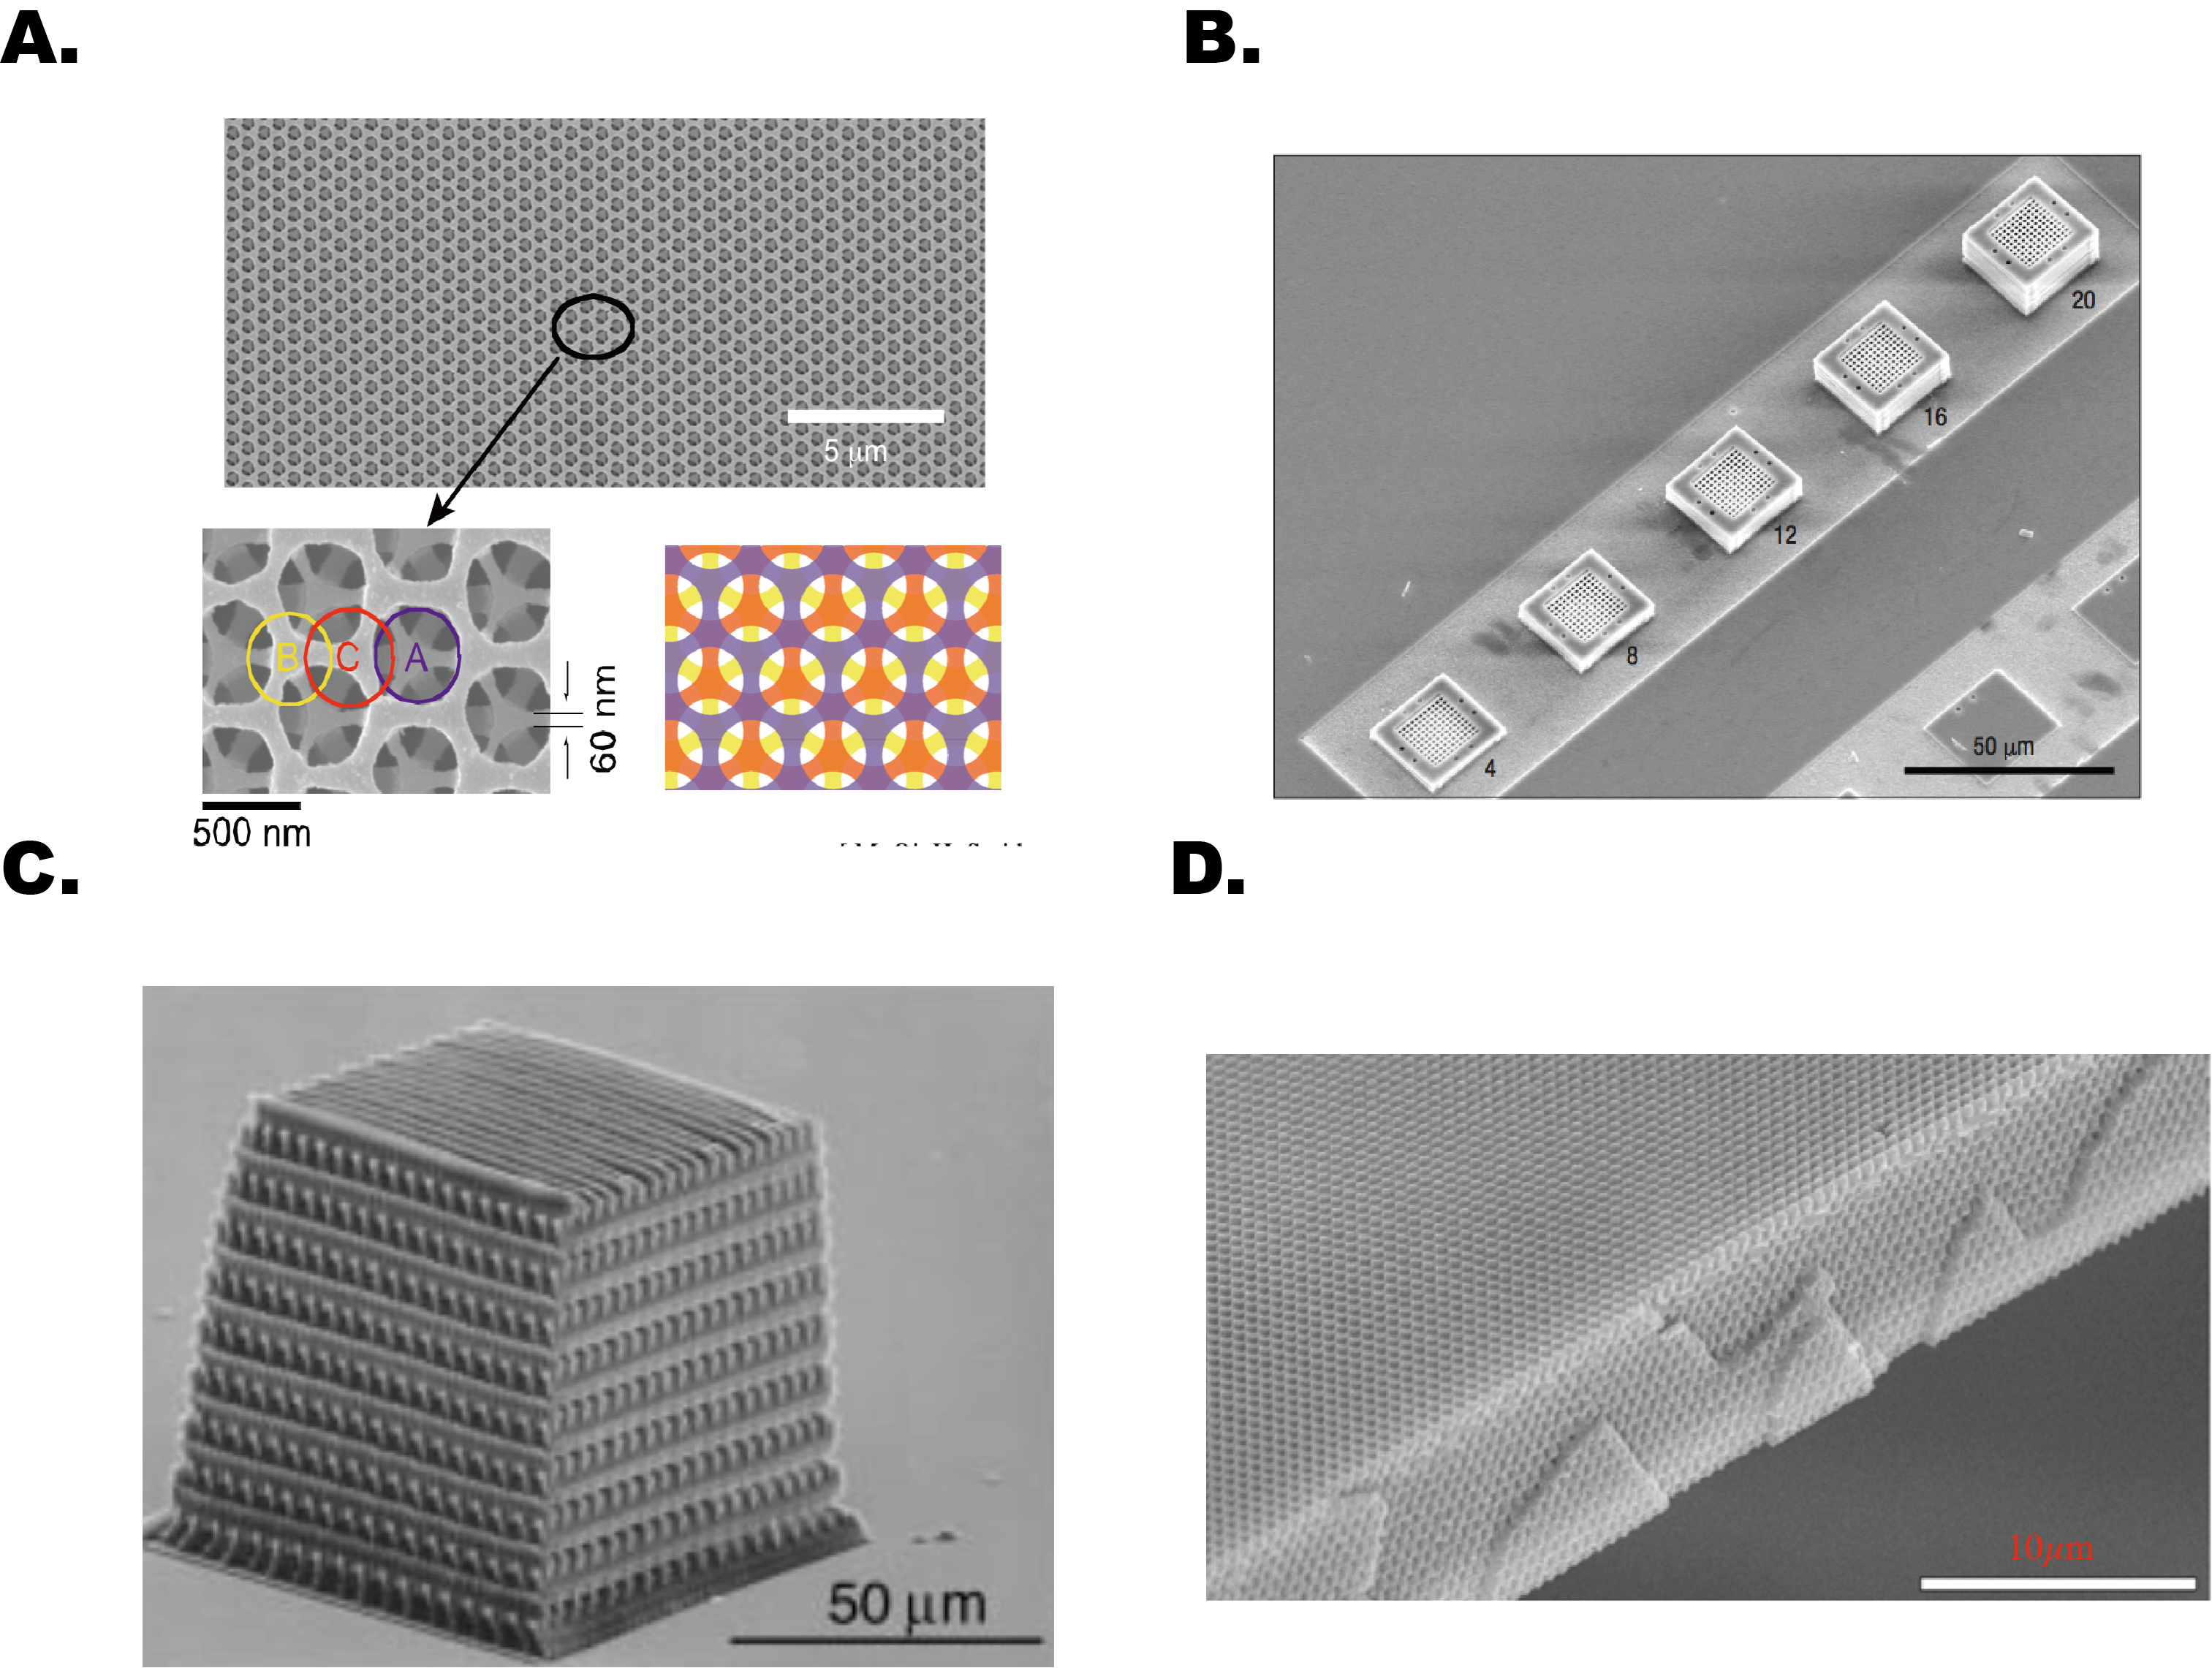
\includegraphics[width=0.8\linewidth]{figures/physPrepare.png}
	\caption{通过物理刻蚀法制备的光子晶体。A.逐层电子束刻蚀\cite{Qi2004ThreeDimensional};B.LbL-电子束刻蚀方法\cite{Aoki2003Microassembly};C.双光子刻蚀\cite{Cumpston1999TwoPhoton};D.单光子全息刻蚀\cite{Campbell2000Fabrication}}
	\label{fig:3DPhysPrepare}
\end{figure}

(3)自组装法

物理刻蚀法主要采用人工方法自上而下制备三维光子晶体材料,而相对应的可以利用
自组装法自下而上(bottom-up),由相分离、重力、电场作用力、毛细作用力等
作用力形成三维光子晶体材料。在小分子材料方面,嵌段高分子是一种非常优秀的
光子晶体构筑材料。通过不同嵌段间的相分离自组装过程,嵌段高分子能够形成一维
至三维尺度上的光子晶体材料\cite{Fink1999Block}。嵌段高分子的组装行为可以通过多相间的比例等参数来进行调节。目前应用较多的为层状组装的嵌段高分子
一维光子晶体\cite{Kang2009Full,Miyake2012Synthesis}。在三维组装上嵌段高分子能够形成如Im${\bar 3}$m、Pn${\bar 3}$m、Ia${\bar 3}$d等特殊晶胞结构,并可以通过进一步处理得到更为复杂的结构\cite{Hsueh2010Inorganic,Hsueh2014Shifting},这是其他方法无法达到的(图~\ref{fig:copol})。但嵌段高分子设计复杂,尤其是三维组装结构较难制备,同时多相之间差异较小,应用有一定限制。
\begin{figure}[htbp]
	\centering
	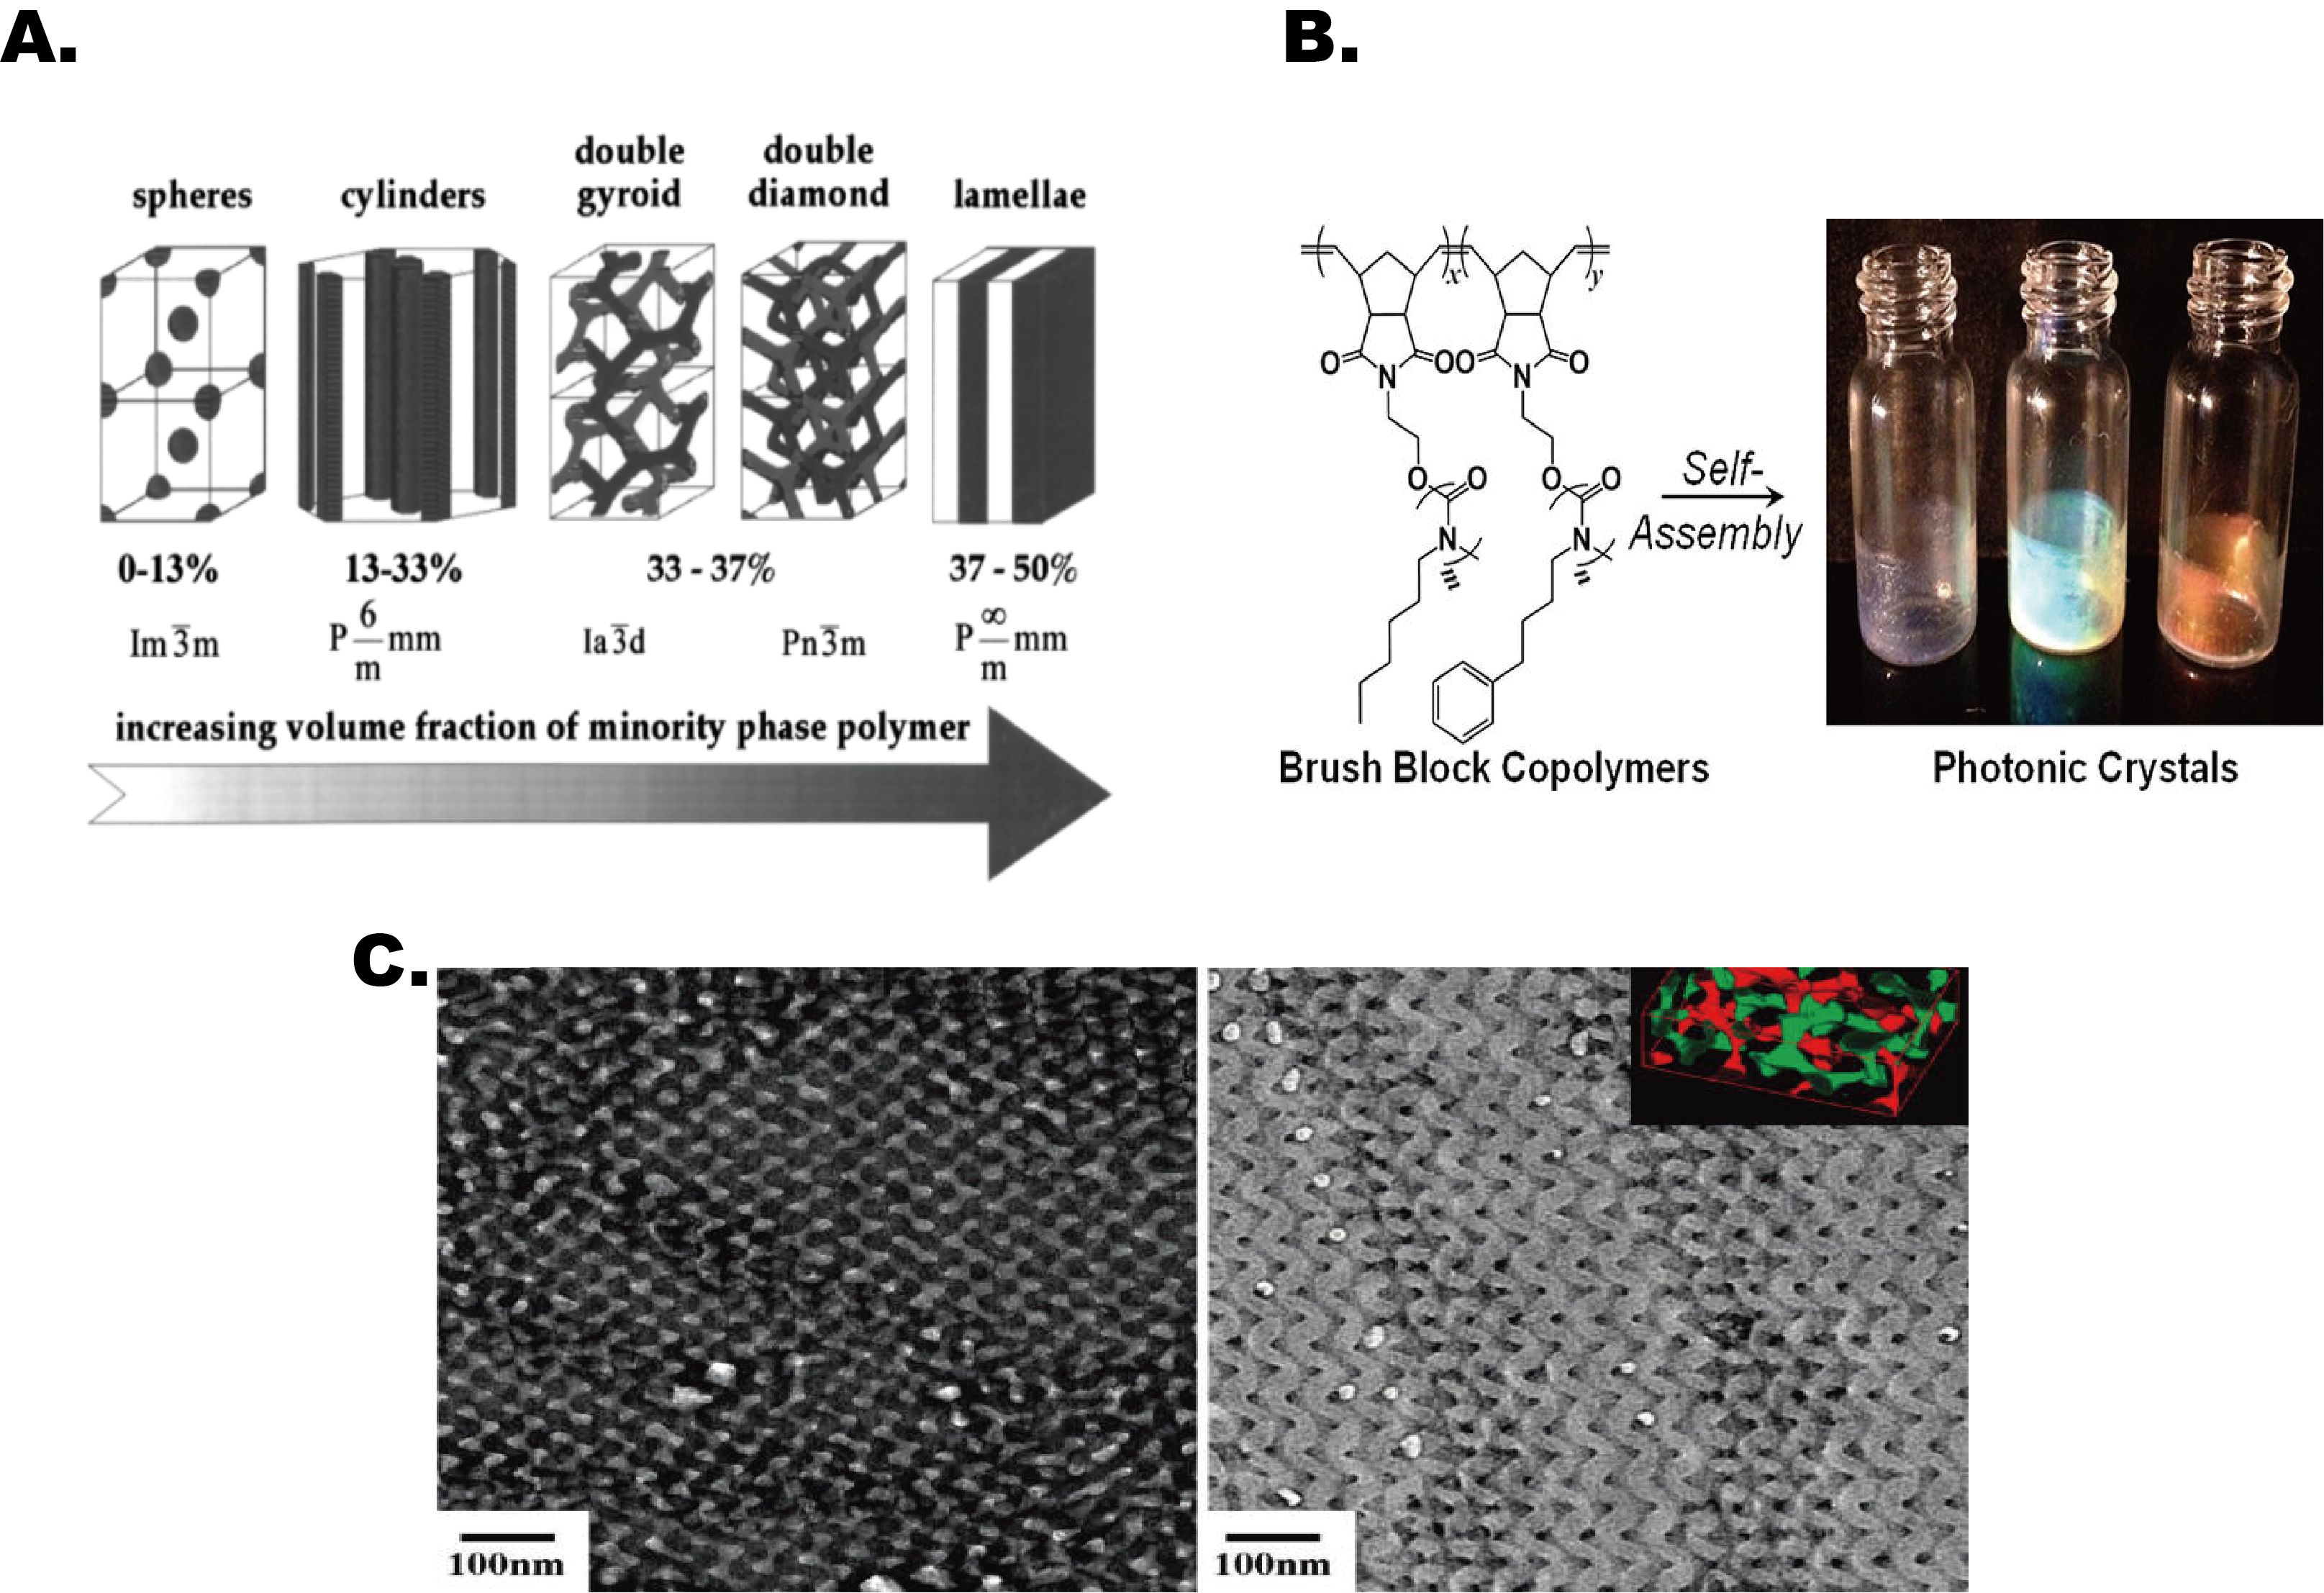
\includegraphics[width=0.8\linewidth]{figures/copol.png}
	\caption{通过嵌段高分子相分离制备光子晶体。A.嵌段高分自组装示意图\cite{Fink1999Block};B.嵌段高分自组装形成的一维光子晶体\cite{Miyake2012Synthesis};C.嵌段高分子形成的Ia${\bar 3}$d三维光子晶体\cite{Hsueh2010Inorganic}}
	\label{fig:copol}
\end{figure}

胶体颗粒的自组装是当前自下而上制备光子晶体的主要手段。早在20世纪60年代
人们便发现蛋白石的结构色来自于其中有序排列的单分散二氧化硅纳米颗粒\cite{Darragh1966Origin,Iler1965Formation},并由此开展了胶体颗粒组装方法的研究。
早期常用垂直沉降法进行制备\cite{Darragh1970Opaline},这种方法能够生长较大尺寸的光子晶体,
但耗时且机械性能差。目前较常用毛细作用诱导的垂直沉积法来制备较高质量的三维光子晶体\cite{Jiang1999SingleCrystal}。这种方法的工艺与材料来源均很简单,能够较好
控制光子晶体的厚度,但同时界面移动形成的缺陷不可避免,且需要较长生长时间。
利用在胶体分散液中加入硅烷前驱体则能够制备几乎无缺陷的二氧化硅反蛋白石光子晶体\cite{Hatton2010Assembly}。与毛细作用相似的也可以利用界面组装制备三维光子晶体。Fudouzi等利用水相胶体分散液与硅油的界面进行聚苯乙烯(PS)与
二氧化硅小球的组装\cite{Fudouzi2004Fabricating,Fudouzi2007Novel},随着水相界面在挥发时的均匀收缩而形成高质量大面积光子晶体。类似地,Jiang等利用超疏水表面上液面的均匀挥发也获得了窄禁带的光子晶体\cite{Huang2012Colloidal}。
同时,利用液滴界面的组装能够获得一系列非平面的三维光子晶体材料。利用喷墨打印技术
可以在基板上形成光子晶体点阵\cite{Cui2009Fabrication,Wang2012Inkjet}。
此外,利用含胶体颗粒的微流控液滴在油相的挥发组装能够制备光子晶体微球\cite{Sun2008Fabrication,Zhao2014Spherical}。
由于其球形对称性,光子晶体微球具有独特的角度不依赖性\cite{Gu2013Tailoring}。上述基于溶剂挥发形成光子晶体的方法总结见图~\ref{fig:evap_opal}。
\begin{figure}[htbp]
	\centering
	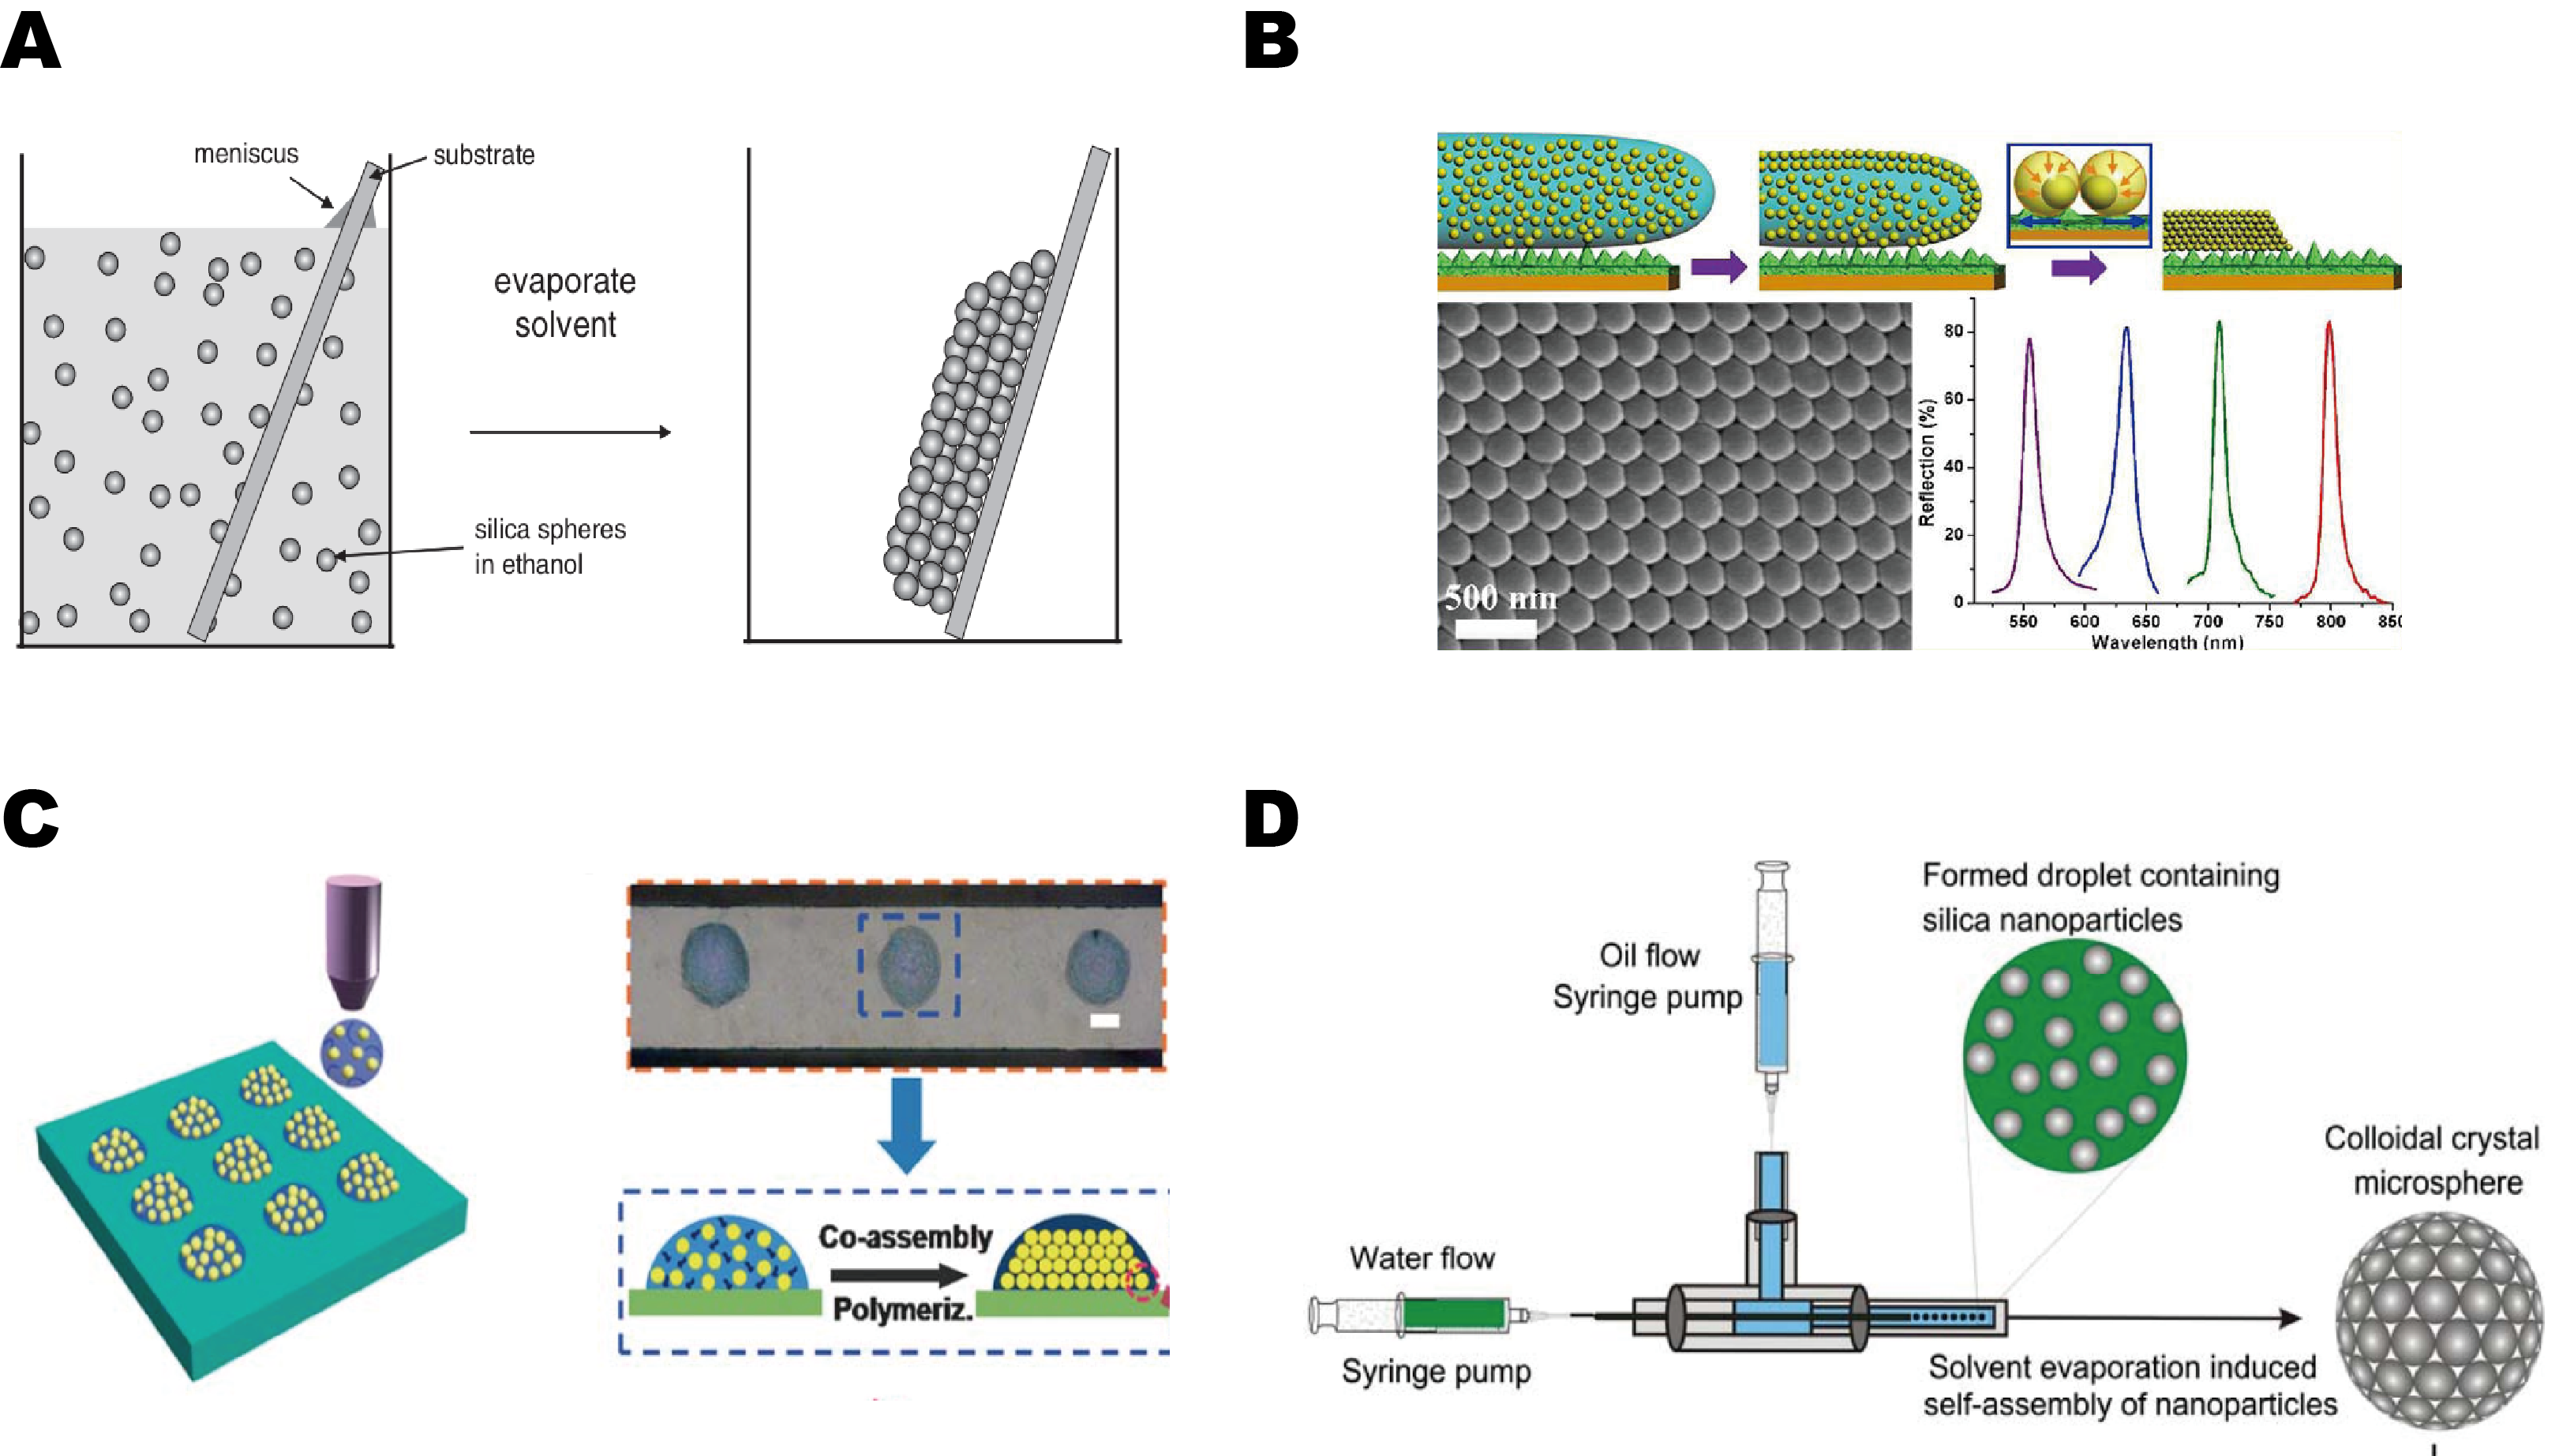
\includegraphics[width=0.8\linewidth]{figures/evap-opal.png}
	\caption{通过溶剂挥发组装制备光子晶体。A.毛细作用诱导的垂直沉积法\cite{Norris2004Opaline};B.超疏水表面组装形成高质量光子晶体\cite{Huang2012Colloidal};C.喷墨打印形成三维光子晶体阵列\cite{Wang2012Inkjet};D.微流控液滴挥发组装形成光子晶体微球\cite{Cui2014Inverse}}
	\label{fig:evap_opal}
\end{figure}

此外,Asher等利用带电荷胶体球在超纯水中的静电力组装制备了非紧密堆积的三维光子晶体及其水凝胶复合物\cite{Lee2000Photonic,Muscatello2008PolyVinyl}。
Jiang等也利用旋涂过程中的溶剂剪切力来进行胶体颗粒的组装,形成大面积的光子晶体材料\cite{Jiang2004LargeScale}。
但需要主要的是上述方法制备的光子晶体为非紧密堆积的光子晶体,在制备其反蛋白石结构及传感响应方面均有一定局限,且技术难度大于溶剂挥发自组装方法。其他制备光子晶体的方法如液面切割法\cite{Yang2010LargeScale}、电沉积法\cite{Arpin2011Electrodeposited}、电喷雾法\cite{Shen2010Fabrication}等这里简略不述。

与物理刻蚀法的人为制备理念不同,自组装法主要依赖高分子或胶体在自然作用力影响
下形成的规整组装结构来制备光子晶体。这类方法在成本和时间消耗上均具有优势。
尽管晶体缺陷在自组装法中难以避免,但由于光子晶体自身的均质性,
其宏观的光子禁带结构受影响并不大。这也使得自组装法在光子晶体的制备中获得了广泛的应用。

\section{光子晶体在传感方面的应用}
\label{sec:PhC-sensing}

\ref{subsec:3DPhC}节中介绍了光子晶体的光学性质随其内在结构参数之间的变化关系。
可以将这种自表达的光学信号平台作为很好的化学或生物传感单元。本节中将简要介绍基于
不同机理的光子晶体传感应用。

\subsection{基于响应性高分子的三维光子晶体材料}
\label{subsec:ion-response}
响应性高分子在不同外界刺激下下体积变化可以带来光子晶体结构参数$D$的变化,从而带来光子晶体的禁带变化。Asher等通过水凝胶型胶体晶体阵列(photonic colloidal crystal array,PCCA)制备了一系列对离子及小分子传感应用。
利用冠醚修饰的丙烯酰胺凝胶可以对Pb\text{$^{2+}$}进行响应\cite{Reese2001Development}。利用多酚基团可以对Ni\text{$^{2+}$}、Co\text{$^{2+}$}、Cu\text{$^{2+}$}、Zn\text{$^{2+}$}等离子进行响应\cite{Asher2003Photonic}。
类似地,利用聚丙烯酸(poly acrylic acid,PAA)或聚羟乙基甲基丙烯酸酯(P-HEMA)水凝胶材料的PCCA可以作为pH与粒子强度的传感器\cite{Lee2000Photonic,Xu2008Polymerized}。
利用含苯硼酸基团的光子晶体材料则可以对葡萄糖浓度进行响应\cite{Honda2009Confined}。

除了对溶质的传感应用之外,基于响应性高分子的光子晶体材料还能够用于对一系列物理
参数进行传感。Takeoka等利用聚N-异丙基丙烯酰胺(P-NIPAM)在临界最小会溶温度(LCST)附近的水分变化制备了光子晶体温度传感器\cite{Takeoka2002Polymer,Matsubara2007Thermally}。光子晶体的禁带特性赋予了其裸眼检测的优势。此外还有利用弹性高分子制备的力传感光子晶体\cite{Wang2014Robust,Scheid2014Redox},使得力学信号能够直观地反映为光子晶体的颜色变化。基于响应性高分子的三维光子晶体材料小结见图~\ref{fig:responsive_phC}。
\begin{figure}[htbp]
	\centering
	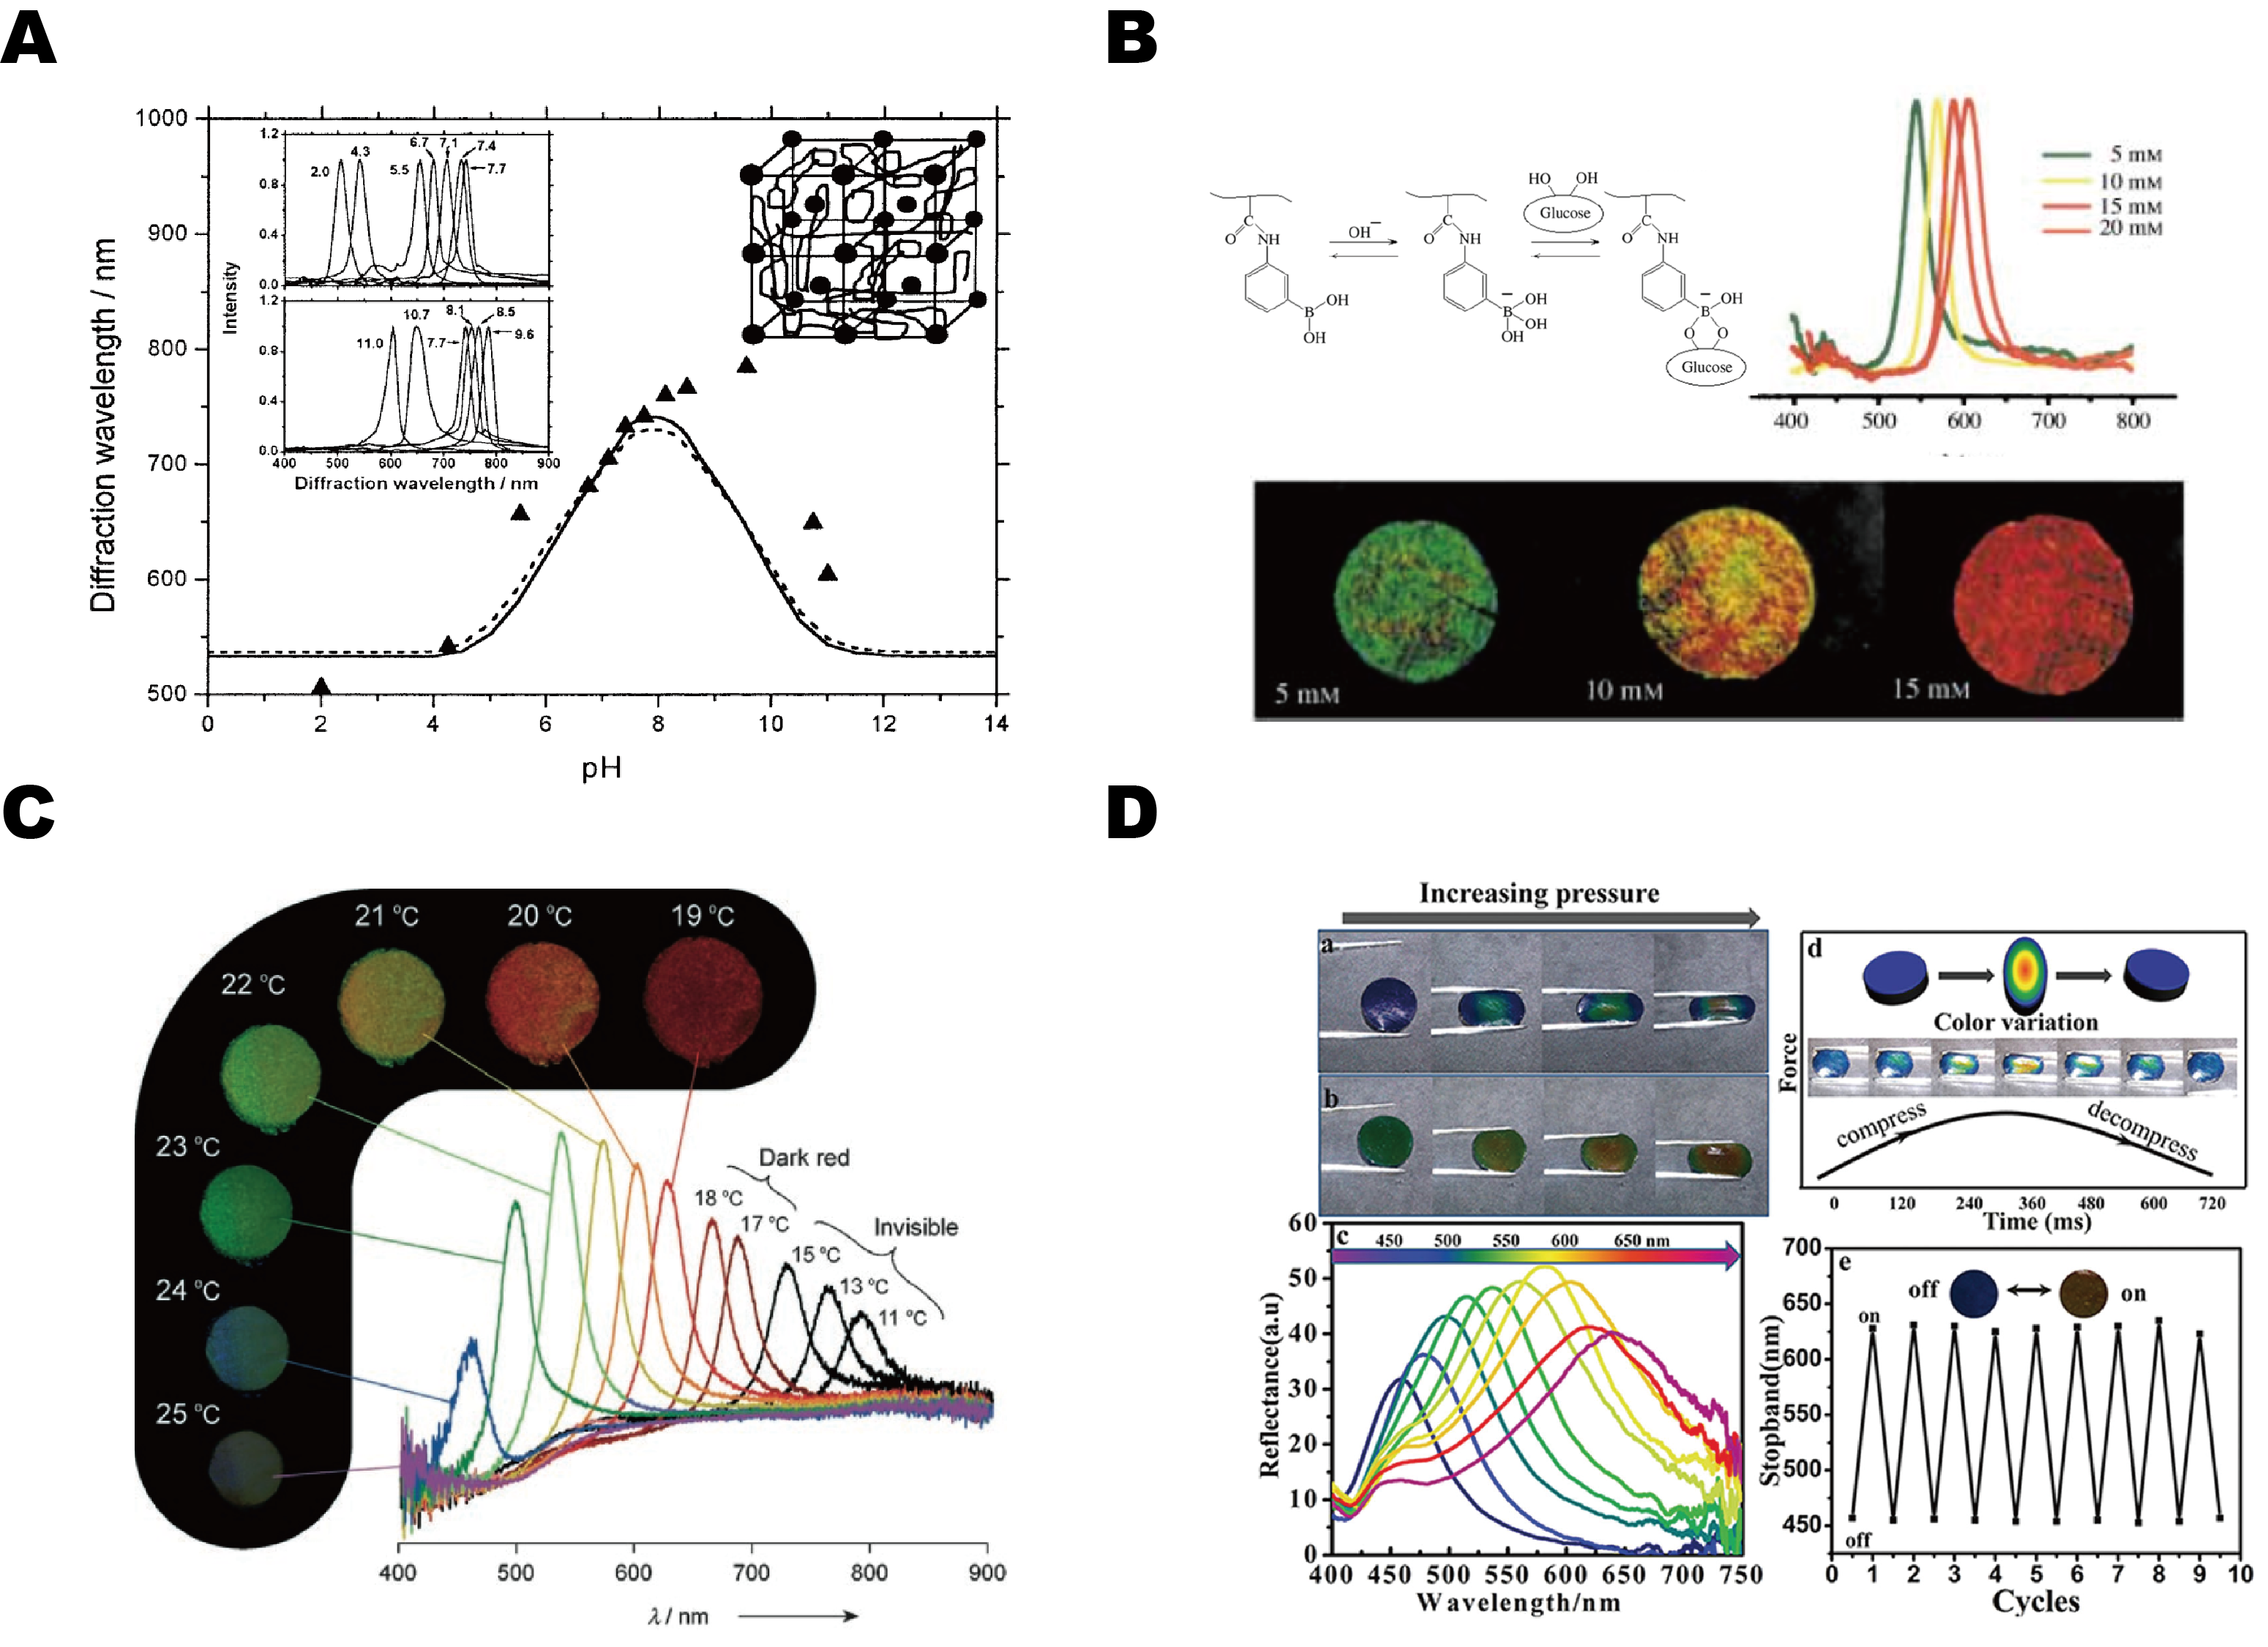
\includegraphics[width=0.8\linewidth]{figures/responsive-pol-PhC.png}
	\caption{基于响应性高分子的光子晶体传感应用示例。A.对pH值的传感\cite{Lee2000Photonic};B.对葡萄糖浓度的传感\cite{Honda2009Confined};C.对温度的传感\cite{Matsubara2007Thermally};D.对机械力的传感\cite{Wang2014Robust}}
	\label{fig:responsive_phC}
\end{figure}

\subsection{基于分子印迹的三维光子晶体材料}
\label{subsec:mol-imprint}

响应性高分子在光子晶体中具有巨大的潜在用途,但其对不同的物质进行传感时需要进行
一定的官能团设计,对于没有特殊位点的物质很难找到匹配的体系。利用分子印迹与光子晶体平台进行结合能够很好地解决这些问题。利用多重非特异性作用力使目标化合物与高分子
之间形成的“锁—钥”结构,
能够使分子印迹后的光子晶体对目标化合物有着很好的特异性识别。
基于这一原理本课题组实现了对多种化合物的检测传感,包括多肽\cite{Hu2007Construction}、兴奋剂\cite{Hu2008Ultrasensitive}、除草剂\cite{Wu2008LabelFree}、多溴苯醚\cite{Xu2014LabelFree}等(图~\ref{fig:mol_imprint})。
更为特别地,这种分子印迹与光子晶体结合的传感方法能够很好地对手性物质\cite{Hu2006Imprinted}以及实际样品\cite{Xu2014Molecularly}进行检测,大大提高了光子晶体传感的使用范围。
\begin{figure}[htbp]
	\centering
	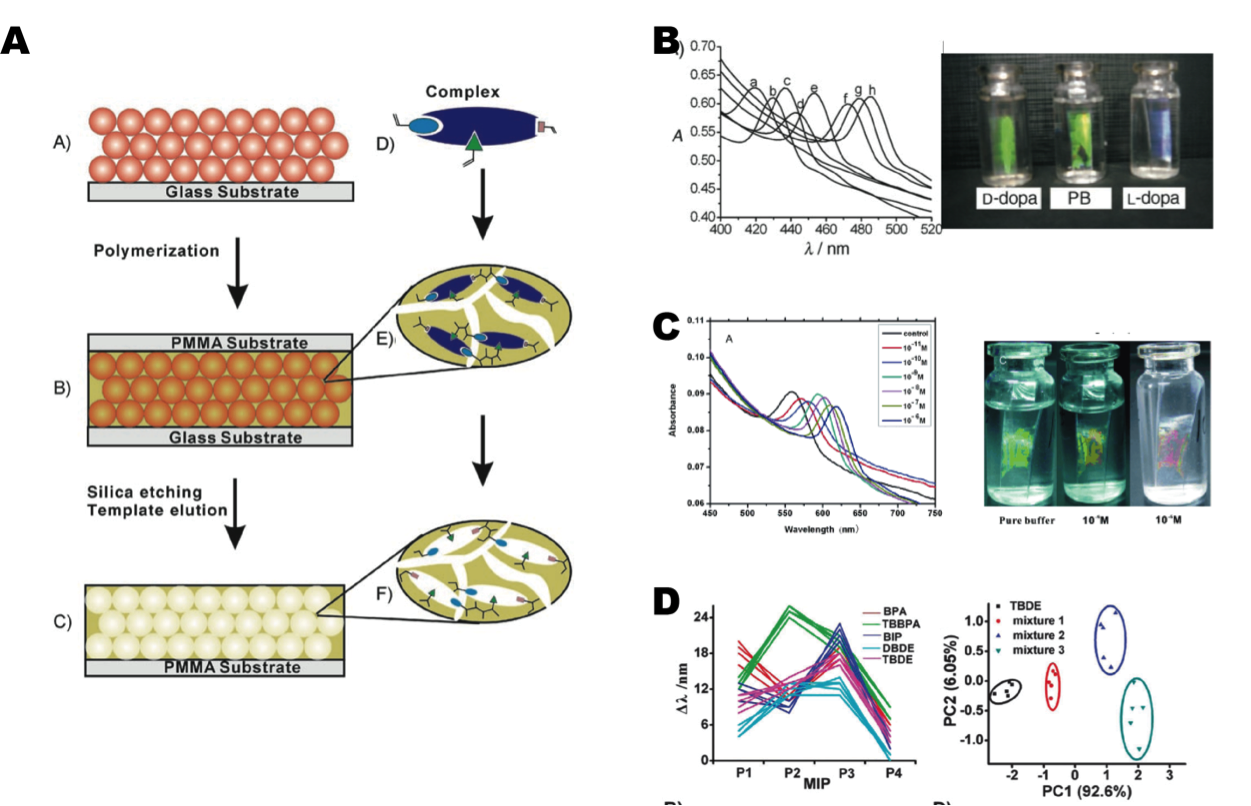
\includegraphics[width=0.8\linewidth]{figures/mol-imprint.png}
	\caption{基于分子印记的光子晶体传感应用示例。A.分子印记光子晶体的原理;B.对手性分子的识别\cite{Hu2006Imprinted};C.对除草剂的识别\cite{Wu2008LabelFree};D.对多溴苯醚的识别与分离\cite{Xu2014LabelFree}}
	\label{fig:mol_imprint}
\end{figure}

\subsection{基于化学反应的三维光子晶体材料}
\label{subsec:chem-reaction}

尽管响应性高分子或分子印迹技术能够获得很好的传感特性,但对于单体设计及聚合条件控制的要求较高,并且有部分功能基团并不能在高分子聚合的过程中稳定存在。需要寻求一系列具有可拓展性及反应性的光子晶体材料来克服上述问题。因此近年来本课题组发展了一系列基于化学反应的光子晶体材料。
由于光子晶体材料的三维有序结构很容易在苛刻的条件(如高温、高热、酸碱性)条件下
被破坏,因此在光子晶体上进行的化学反应必须是温和且快速的。Sharpless等提出的“点击化学”(click chemistry)反应\cite{Kolb2001Click}则以其高效、快速及温和的特性而满足上述要求。
Li等通过三氟乙酰苯胺官能团与CN\text{$^-$}的S\text{$_N$}2反应,制备了对CN\text{$^-$}离子响应的光子晶体,并用于检测水相中的有毒CN\text{$^-$}残留,能够达到10\text{$^{-7}$} mol/L级别的检测限\cite{Li2012Reactive}。
Xu等利用合成了含叠氮基团的反蛋白石光子晶体,并通过Cu(I)催化的叠氮-炔基点击反应在光子晶体平台上进行后修饰\cite{Xu2012Clickable}。
通过这种方法能够将普通的光子晶体平台拓展为具有电化学活性、pH响应性、溶剂响应性及生物相容性的光子晶体材料。
类似地,利用马来酰亚胺官能团与巯基化合物的Michael加成反应及与共轭二烯化合物的[4+2]Diels-Alder加成反应,可以将光子晶体变为具有更多拓展性的平台。
Yang等利用基于马来酰亚胺的光子晶体平台将其拓展为具有电化学活性、pH响应性、生物巯基化合物检测以及动态开关体系的功能材料\cite{Yang2013MaleimideContaining}。

除了点击反应之外,离子液体的对抗离子交换反应也被应用于基于化学反应的光子晶体材料。
通过对抗离子交换,能够很好地对离子液体聚合物的亲疏水性、磁性、氧化还原性、催化性等性质进行调控。Huang等通过聚咪唑基离子液体与光子晶体结合,通过不同阴离子交换后的光子晶体禁带的变化实现了对阴离子的识别以及分子通道的应用\cite{Huang20103DOrdered}。
同时,这种聚离子液体光子晶体能对空气中的湿度也有很好的响应性,能够作为裸眼的湿度感应材料\cite{Huang2010Visual}。
当聚离子液体与光子晶体微球相结合时能够更为独特的应用\cite{Cui2014Inverse}。
由于光子晶体微球自身的独立性,能够作为传感阵列来对不同的溶剂进行区分。
同时,这种光子晶体微球能够通过离子交换变为磁性、催化活性、生物活性的大孔微球材料。最后,通过纳米微压印技术能够对光子晶体进行局部修饰,从而制备各向异性的光子晶体微球。

基于化学反应的光子晶体的小结见图~\ref{fig:chem_react_phc}。
\begin{figure}[htbp]
	\centering
	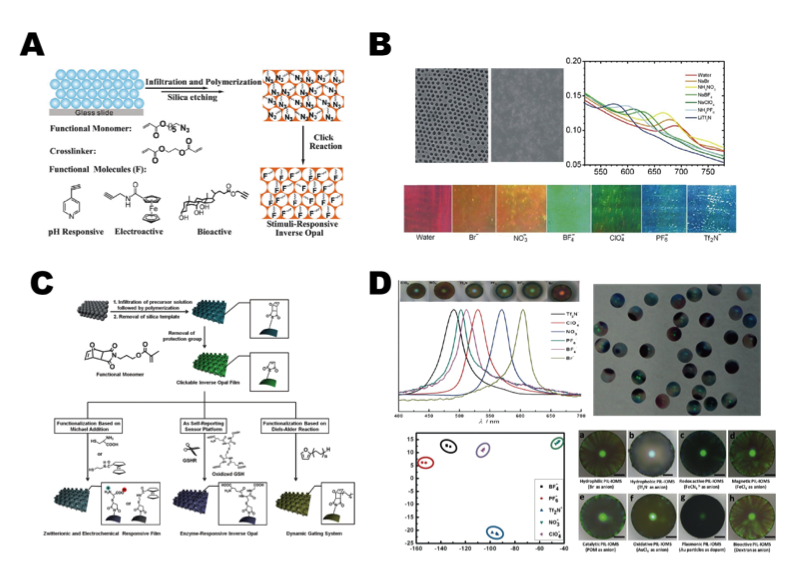
\includegraphics[width=\linewidth]{figures/chem_react_phc.png}
	\caption{基于化学反应的光子晶体传感应用示例。A.利用叠氮-炔基点击反应的活性光子晶体\cite{Xu2012Clickable};B.基于离子液体阴离子交换的光子晶体传感器\cite{Huang20103DOrdered};C.基于马来酰亚胺的活性光子晶体\cite{Yang2013MaleimideContaining};D.基于离子液体的活性反蛋白石光子晶体微球\cite{Cui2014Inverse}}
	\label{fig:chem_react_phc}
\end{figure}
基于化学反应的光子晶体材料赋予了光子晶体更大的拓展性,不仅可以通过化学反应来对特征分子进行识别,更可以通过化学反应将光子晶体后修饰为多功能材料。同时,基于化学反应的光子晶体材料也表现出了向各向异性功能化发展的潜力\cite{Cui2014Inverse},这也是其他功能光子晶体所难以实现的。


\section{多层次光子晶体的制备与研究}
\label{sec:multiscale-phc}

作为一种具有重要应用前景的材料,三维光子晶体已经在许多方面展现出其独特的传感性能与识别特性。目前,大多数针对光子晶体识别性质的研究主要着眼于以形成单一的整体材料,对于在同一光子晶体上集成多重功能结构或层次的研究尚比较少。这种对光子晶体图案化、复杂化、多层次化的研究对显示应用、光子晶体阵列等领域都具有非常重要的意义。本节中将目前报道的光子晶体多层次化的技术进行简要介绍。

\subsection{基于基质膨胀的光子晶体层次化技术}
\label{subsec:matrix-swell}

平面型的复合型光子晶体可以通过局部基质改变的方法来实现图案化。其中最为简便也是常用的方法是对光子晶体的基质进行局部膨胀改变,通过改变膨胀部分的晶格参数$D$来调控局部结构色(图~\ref{fig:matrix_swell})。
\begin{figure}[b]
	\centering
	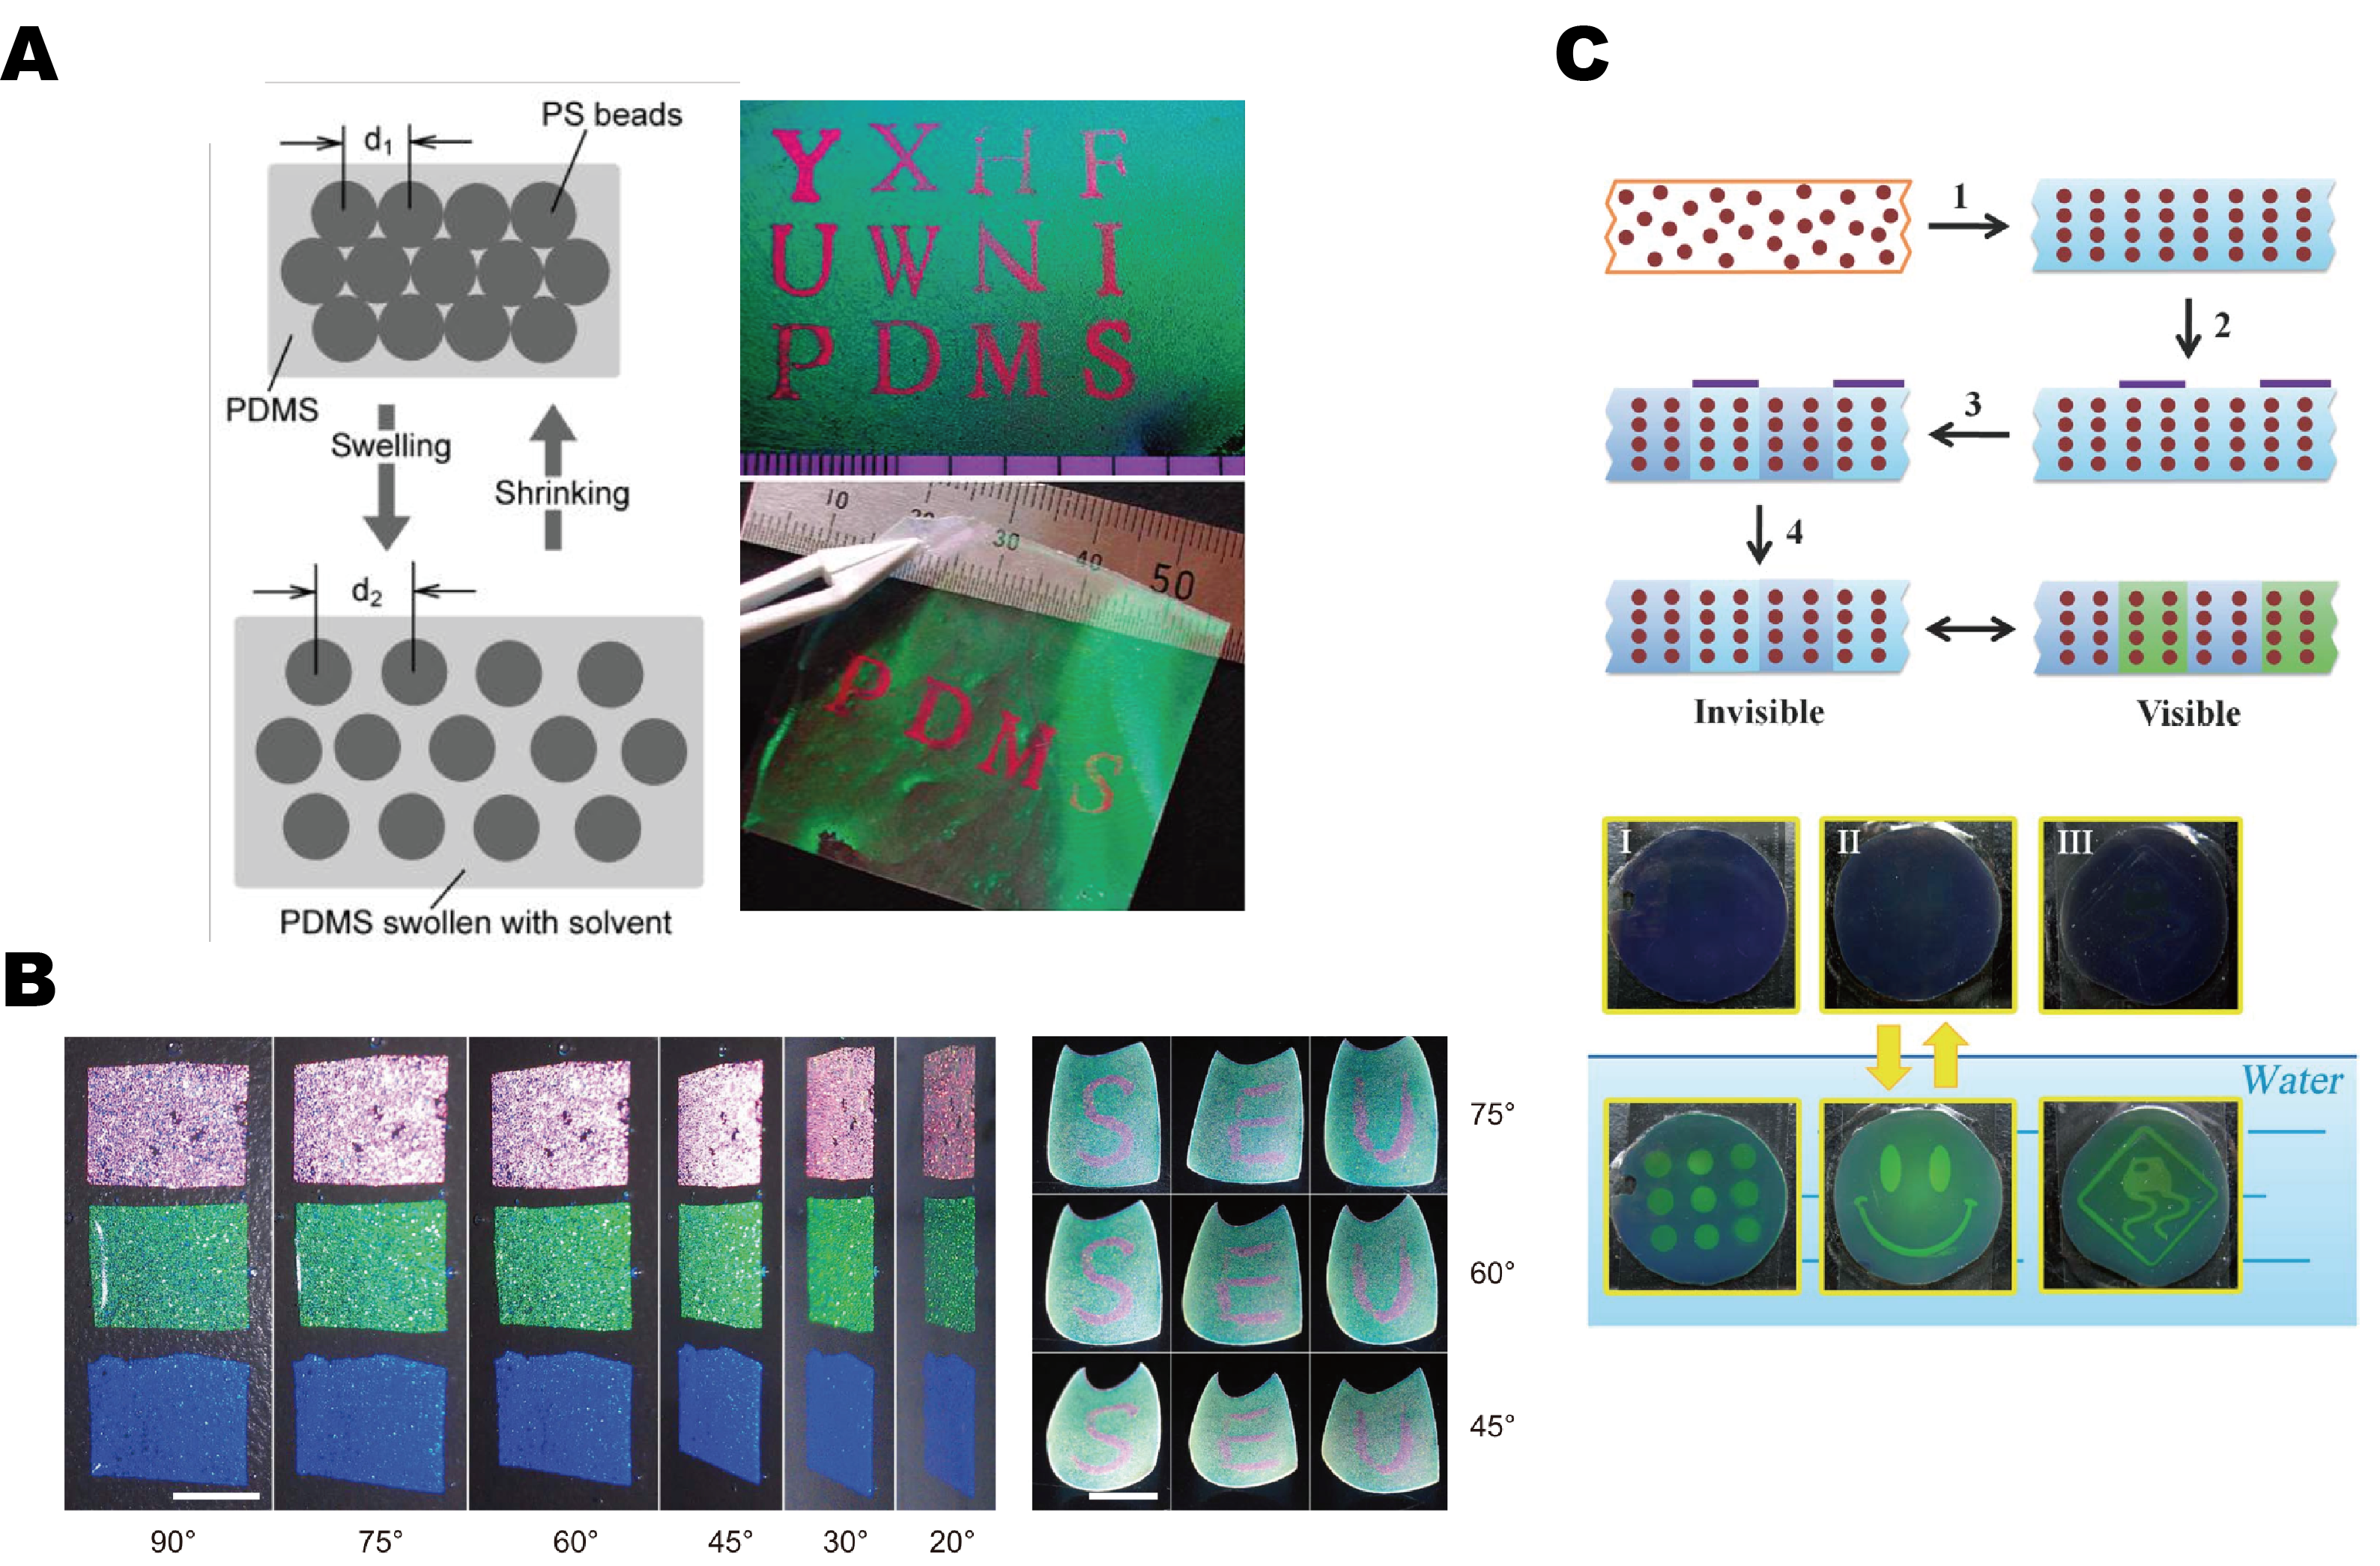
\includegraphics[width=0.9\linewidth]{figures/matrix-swell.png}
	\caption{基于基质膨胀的光子晶体层次化技术示例。A.利用PMDS膨胀的复合光子图案化\cite{Fudouzi2003Colloidal};B.基于光子晶体微球薄膜的角度不依赖图案\cite{Gu2013Tailoring};C.基于基质差异的水显影光子晶体防伪图案\cite{Xuan2011Invisible}}
	\label{fig:matrix_swell}
\end{figure}
Fudouzi等最早报道了通过以PDMS为基质的PS复合光子晶体在硅氧烷溶剂中的体积膨胀来制备可重复读写的光子晶体纸\cite{Fudouzi2003Colloidal}。
通过图章压印技术可以将简单的图案写到这样的光子晶体纸上,由于硅氧烷溶剂不易挥发,因此这种图案化光子晶体具有一定的持久性。类似地,可以通过亲水性高分子光子晶体上压印吸水性盐类的方法来实现亲疏水性图案化擦写\cite{Ge2009Rewritable}。
利用pH响应高分子也能够实现压印图案化\cite{Liu2007Poly4VinylpyridineBased}。同时,利用微米级别的光子晶体微球与亲水高分子组成的光子晶体薄膜能够对压印的水显示图案\cite{Gu2013Tailoring},同时这样的图案也具有角度不依赖性。
上述基质膨胀的方法主要依靠压印方法获得的一次性图案,且由于压印所使用的“墨水”溶液存在扩散,所制得图案精度并不高。

当预先对光子晶体中的部分基质进行处理便可获得稳定的光子晶体图案。
Xuan等通过调控含硅聚合物的不同交联度,制备了随水显影的光子晶体图案\cite{Xuan2011Invisible}。由于在无水的情况下聚合物的折射率相近,图案无法显现;而当聚合物与水作用时,亲水且交联度低的部分能够显示出更高的光子禁带红移,从而显示出所隐藏的图案。这种理念可以很好地应用于光子晶体防伪材料上。

\subsection{基于刻蚀的光子晶体层次化技术}
\label{subsec:etch-pattern}

与自组装光子晶体自下而上的理念相对,刻蚀法是自上而下对已形成的光子晶体进行修饰,由于刻蚀法的高精度特性,这种方法获得的光子晶体层次化结构可以进行精细设计与调控(图~\ref{fig:etch-pattern})。
\begin{figure}[htbp]
	\centering
	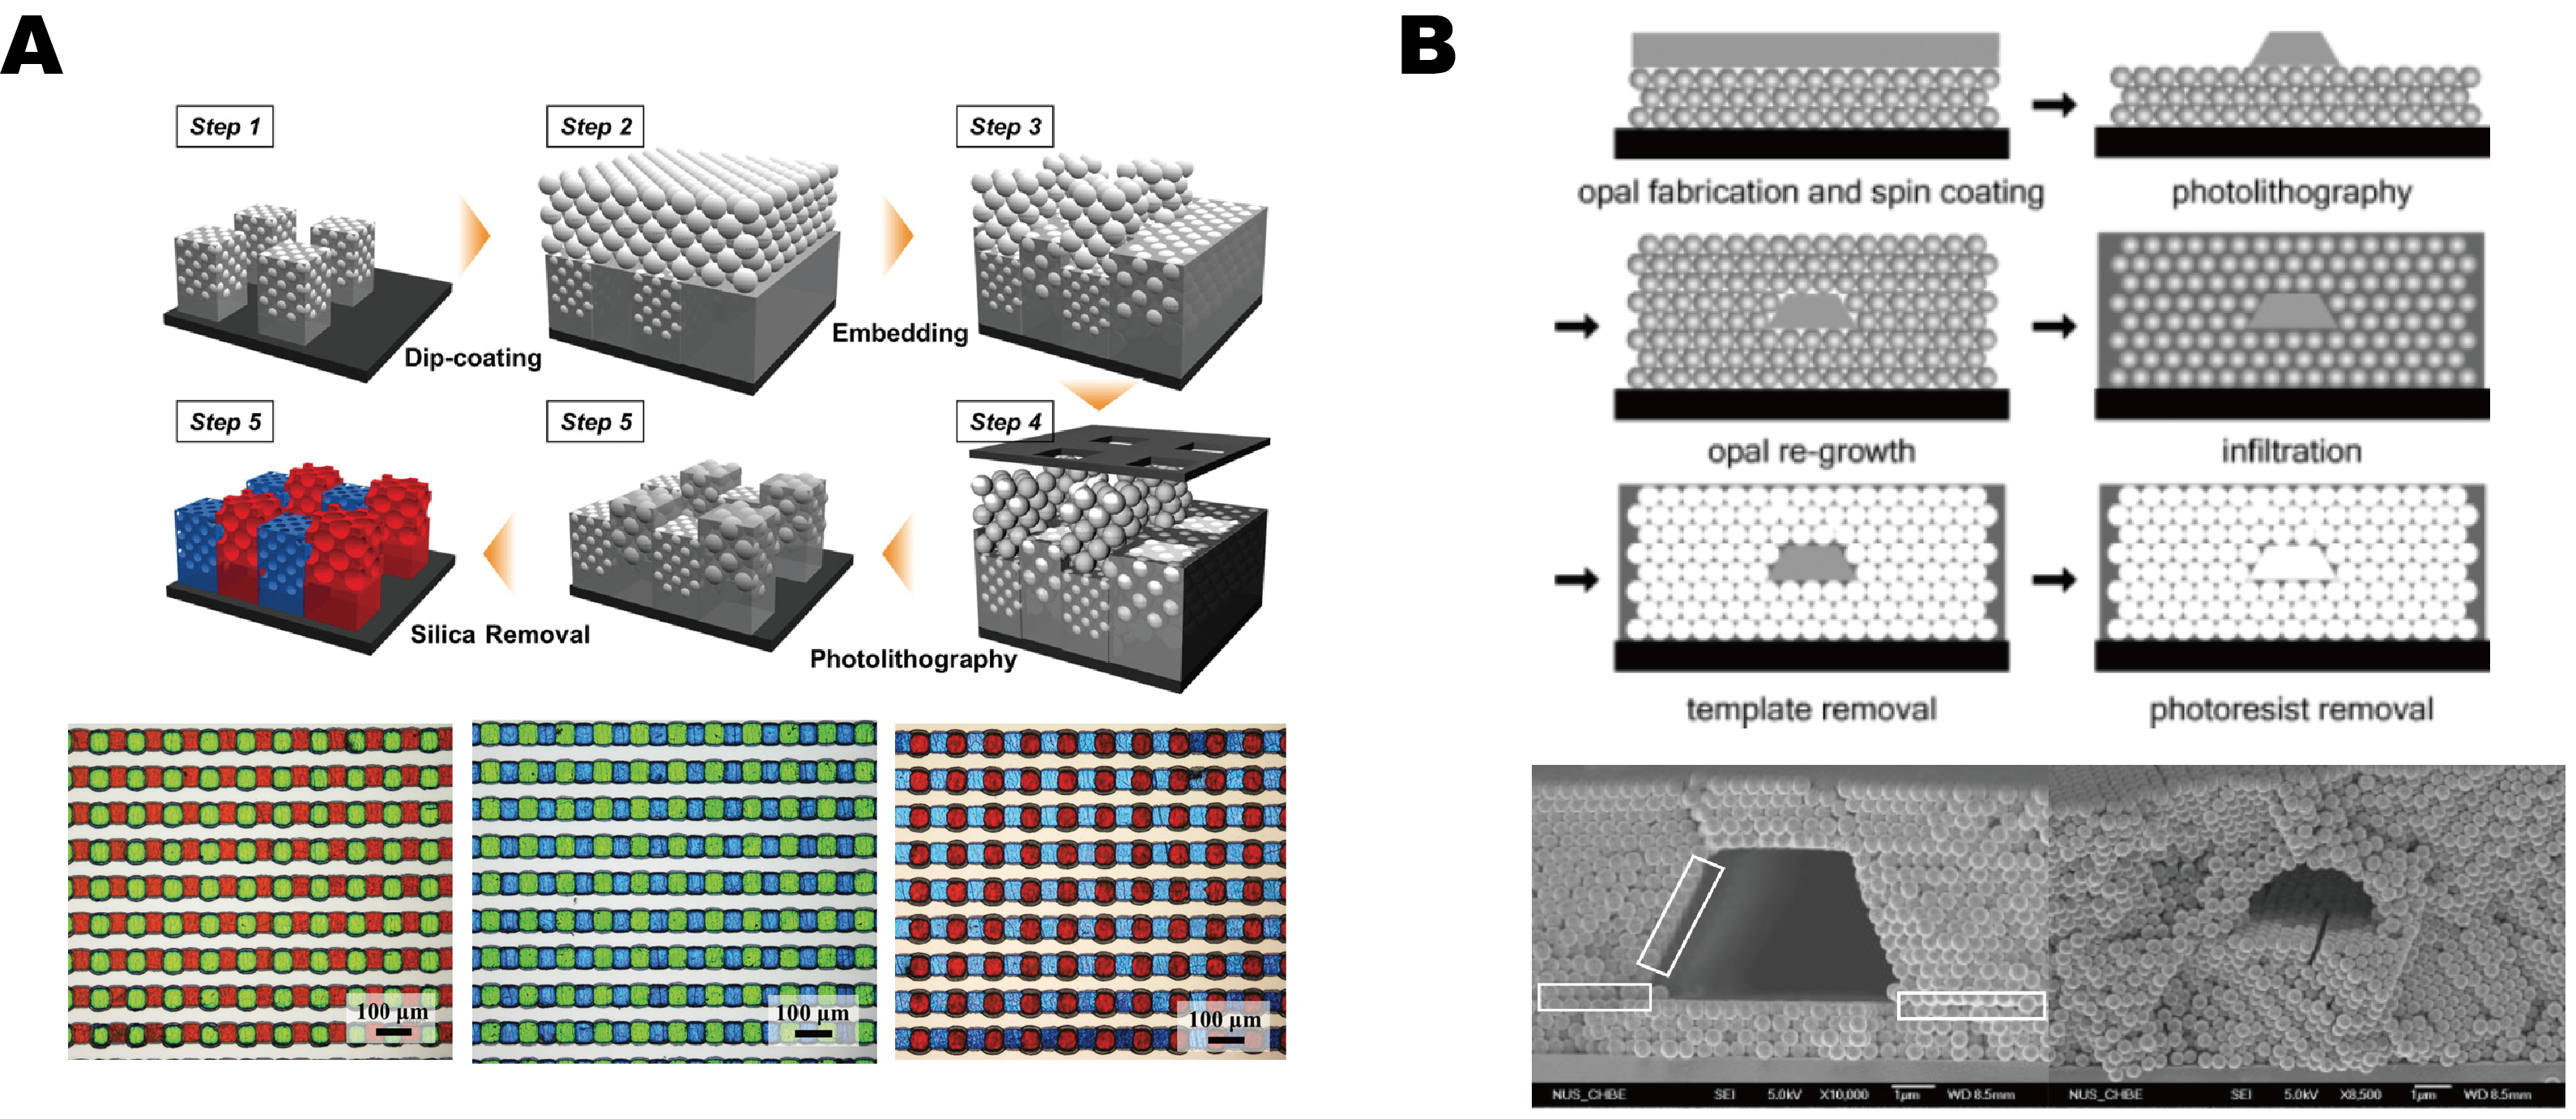
\includegraphics[width=0.9\linewidth]{figures/etch-pattern.png}
	\caption{基于刻蚀的光子晶体层次化技术。A.利用掩膜刻蚀的光子晶体二维图案\cite{Lee2006Pixellated};B.基于刻蚀法的光子晶体三维缺陷设计\cite{Yan2005Line}}
	\label{fig:etch-pattern}
\end{figure}
Lange等选择性光显影对聚甲基丙烯酸叔丁酯(P-tBMA)微球自组装形成的胶体晶体进行图案化刻蚀\cite{Lange2004Photoprocessable}。由于P-tMBA在紫外光下能够释放出羧基基团,因此可以像光刻胶一样制备具有复杂图案的蛋白石型光子晶体模板材料。Lee等通过在SU8光刻胶反蛋白石光子晶体中重新填充SU8并进行反复曝光-显影操作,制备了复杂的光子晶体点阵\cite{Lee2006Pixellated}。同样使用刻蚀与翻模技术能够制备光子晶体点阵或复合结构\cite{Ding2011Patterning,Lee2014Controlled}。
Kang等通过反应离子束刻蚀形成了双层超疏水光子晶体结构,从而获得不随溶剂改变光子禁带的溶剂不通透光子晶体材料\cite{Kang2014LiquidImpermeable}。
同时,通过刻蚀法制备的光子晶体材料并不局限于二维的图案,通过适当方法也可以获得三维的层次结构。Yan等首先在光子晶体表面通过光刻生长立体形状的SU8固体块,并在这种光子晶体上继续进行胶体晶体生长,最终获得了内嵌线缺陷的反蛋白石光子晶体材料\cite{Yan2005Line}。

刻蚀法的优点在于对光子晶体图案的精确调控以及复杂结构的制备。但受刻蚀材料的化学成分限制,光子晶体材料的功能化,尤其是其化学组分的变化较难实现。

\subsection{基于喷墨打印的光子晶体层次化技术}
\label{subsec:inkjet-pattern}

喷墨打印法在制备光子晶体层次化结构上是一种较为直接的方法,可以看作利用光子晶体点阵来实现基质膨胀法或刻蚀法所能实现的光子晶体图案。与文献\onlinecite{Fudouzi2003Colloidal}的原理类似,Kang等通过喷墨打印硅氧烷油滴,在PDMS基的光子晶体纸上打印出线宽达到200 \text{$\mu$}m的图案\cite{Kang2011High}。
说明了喷墨打印法相比于普通方法的精度。此外,也可以利用喷墨打印液滴中胶体颗粒的组装形成光子晶体阵列,例如文献\onlinecite{Cui2009Fabrication}。由于胶体颗粒可以由响应型高分子制备而成,因此可以获得对环境参数(例如温度)响应的光子晶体图案\cite{Wang2012Inkjet},以用于实际应用中。

\subsection{基于电磁场的光子晶体层次化技术}
\label{subsec:magnetelectro-pattern}

电场或磁场作用力也可以用于光子晶体的层次化结构制备。尽管两者的控制方法略有不同,
但原理上都是使用电场或磁场来调控局部胶体组装,从而呈现光子晶体图案(图~\ref{fig:magnet_electro_PhC})。电场控制的光子晶体可以采用在具有氧化还原特性的高分子。例如,Ozin等利用含二茂铁的聚合物复合光子晶体实现了利用电场对光子晶体结构色的调制\cite{Arsenault2007PhotonicCrystal},且能够覆盖全光子禁带。当二茂铁基元在不同电位下呈现出不同的电荷量,从而产生高分子内部的体积变化。当这种随电压改变结构色的材料元器件化之后,能够将其应用于点阵化光子晶体显示器材上。
电场作用需要将光子晶体直接置于电极作用下,需要采用ITO等透明电极材料来实现器件化。而磁场作用则为远程作用,可以通过非接触方式来操纵光子晶体组装。
当具有铁磁性的胶体颗粒(例如Fe\text{$_3$}O\text{$_4$}@SiO\text{$_2$}胶体颗粒)悬浮体系处于磁场作用下,磁性胶体颗粒会形成自动组装的结构,调节其折射率与胶体颗粒体积比则可形成光子晶体\cite{Ge2009Magnetochromatic}。
利用这一原理可以在复杂的磁场条件下进行磁响应光子晶体禁带的调控。He等利用Halbach磁极阵列制造了周期性变化的磁场,并以此进行光子晶体禁带的动态调控\cite{He2011Assembly}。
然而变化的磁场调控较电场更为困难,因此更为实用的方法为利用局部磁场取向光子晶体,进而使用固化法将光子晶体构象稳定,形成持久图案。
Ge等利用不同强度的磁场调控光子晶体禁带颜色并用聚焦紫外将光子晶体固化为显示单色基元点阵;通过多部方式制备了全色系的光子晶体图案\cite{Kim2009Structural}。此外,由于磁响应的光子晶体内部排列具有相位,还可以通过不同磁化角度来调控图案间的相位差,以制备光学防伪材料\cite{Xuan2011Photonic}。
\begin{figure}[htbp]
	\centering
	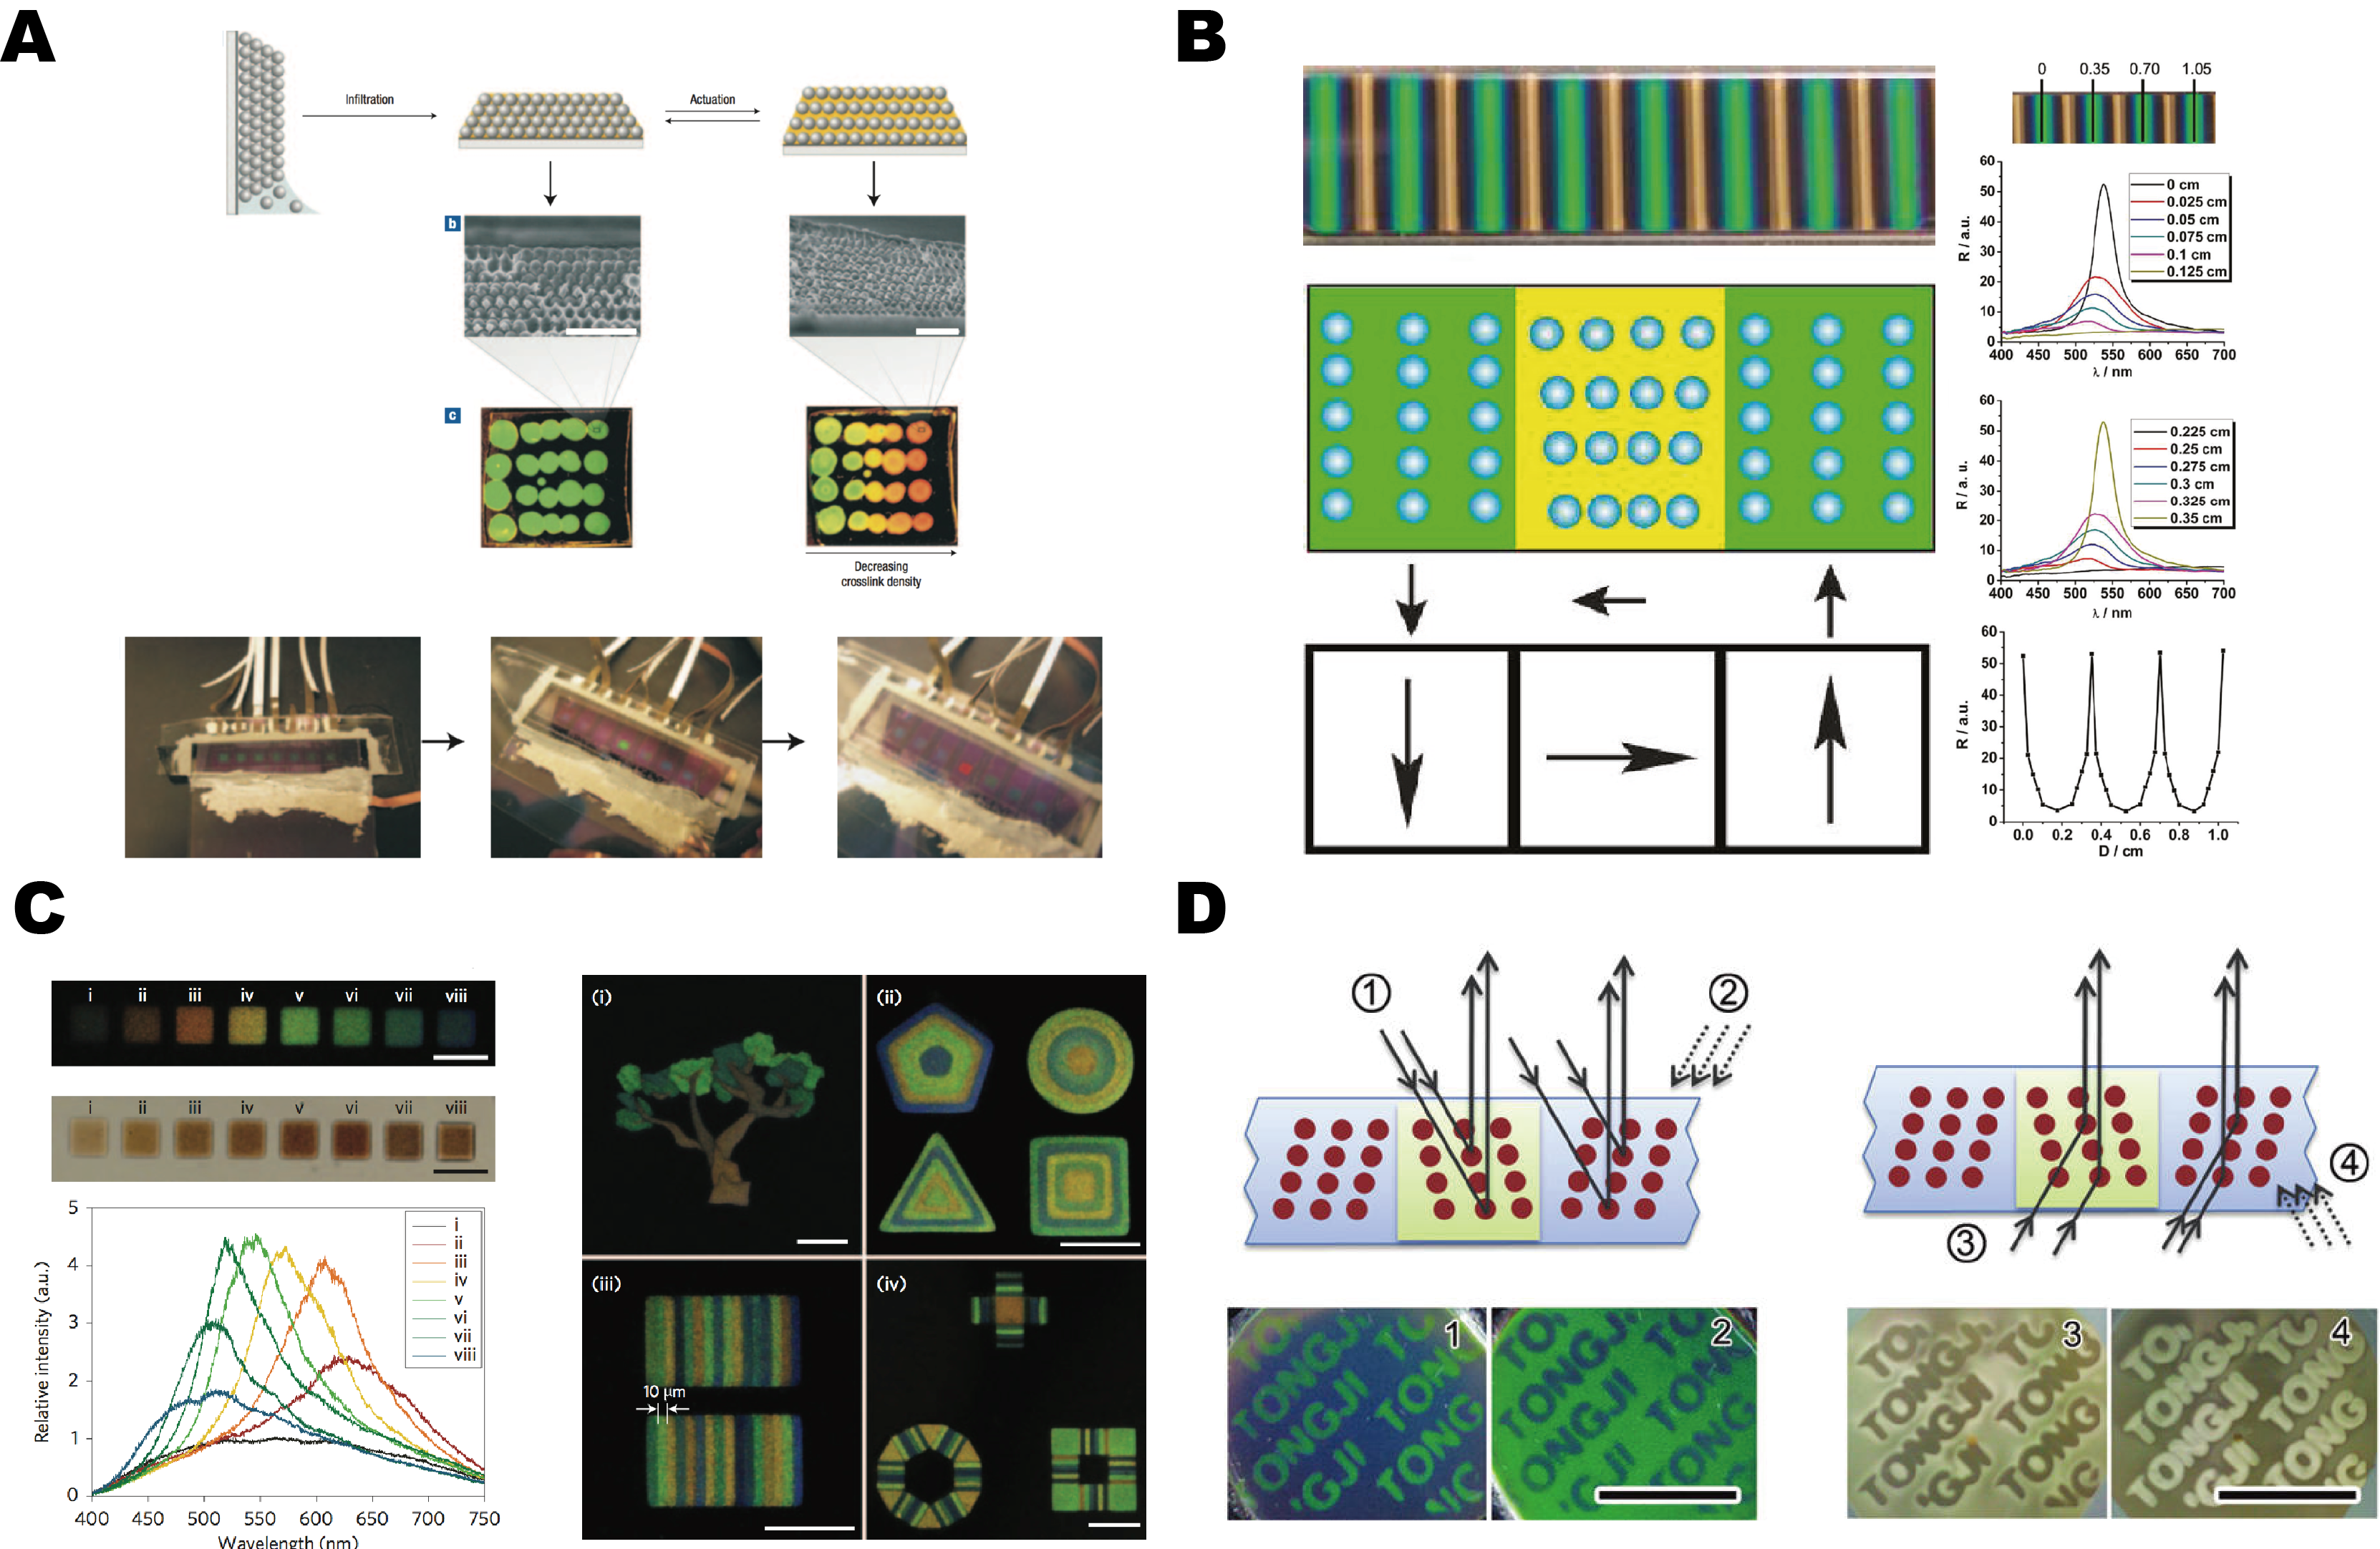
\includegraphics[width=0.9\linewidth]{figures/magnet_electro_phC.png}
	\caption{基于电场或磁场调控的光子晶体层次化技术。A.利用电场调控的光子晶体阵列\cite{Arsenault2007PhotonicCrystal};B.在复杂磁场下调控的光子晶体图案\cite{He2011Assembly};C.利用不同场强磁场逐步固化的光子晶体图案\cite{Kim2009Structural};D.利用不同相位磁场逐步固化的光子晶体图案\cite{Xuan2011Photonic}}
	\label{fig:magnet_electro_PhC}
\end{figure}

\subsection{反蛋白石结构上层次化技术}
\label{subsec:inverse_opal_pattern}

\ref{subsec:matrix-swell}-\ref{subsec:magnetelectro-pattern}节介绍的光子晶体图案化的方法主要主要应用于蛋白石型或复合型的光子晶体材料。
相比之下,在反蛋白石结构上的光子晶体层次化则更具有挑战性。
由于反蛋白石结构自身的一体性,很难利用上述的刻蚀法或喷墨打印法;
同时,由于反蛋白石的连续互穿孔道结构,液体进入光子晶体孔道后便会向各方向扩散,无法实现利用液滴基础控制的基质膨胀图案化法。
然而,蛋白石型的光子晶体材料受限于胶体颗粒材料的制备,而反蛋白石光子晶体则不具有这种限制,可以利用几乎任何可聚合材料进行构筑。
因此反蛋白石结构上的层次化具有非常重要的研究意义。目前针对反蛋白石光子晶体的层次化修饰研究较少,主要可利用的方法包括拓扑聚合法、表面修饰法等(图~\ref{fig:inverse_opal_pattern})。

拓扑聚合的方法主要利用了可控聚合技术,通过多次聚合形成图案化的光子晶体复合结构,最后进行刻蚀以形成具有层次结构的反蛋白石光子晶体材料。Lee等利用掩膜UV聚合方法制备了聚丙烯酰胺凝胶反蛋白石阵列用于蛋白石生物固定\cite{Lee2012Preparation}。
其中,经过UV聚合的丙烯酰胺凝胶固化了反蛋白石结构,而未聚合的部分可以被溶剂洗去,从而形成具有图案化的光子晶体结构。Wang等利用两步的拓扑聚合方法来制备二元反蛋白石光子晶体薄膜\cite{Wang2011Tuning},将具有不同pH响应性的反蛋白石结构整合,形成随pH变化的二元图案。
但拓扑聚合在应用上具有一定的限制。首先,拓扑聚合涉及 多光子晶体材料的反复精细操作,失败率高;其次,UV聚合过程中的自由基扩散也会造成其他部分的聚合,因此这种方法仅适用于少数具有快聚合速度的高分子材料,且不能制备很复杂的图案。
\begin{figure}[htbp]
	\centering
	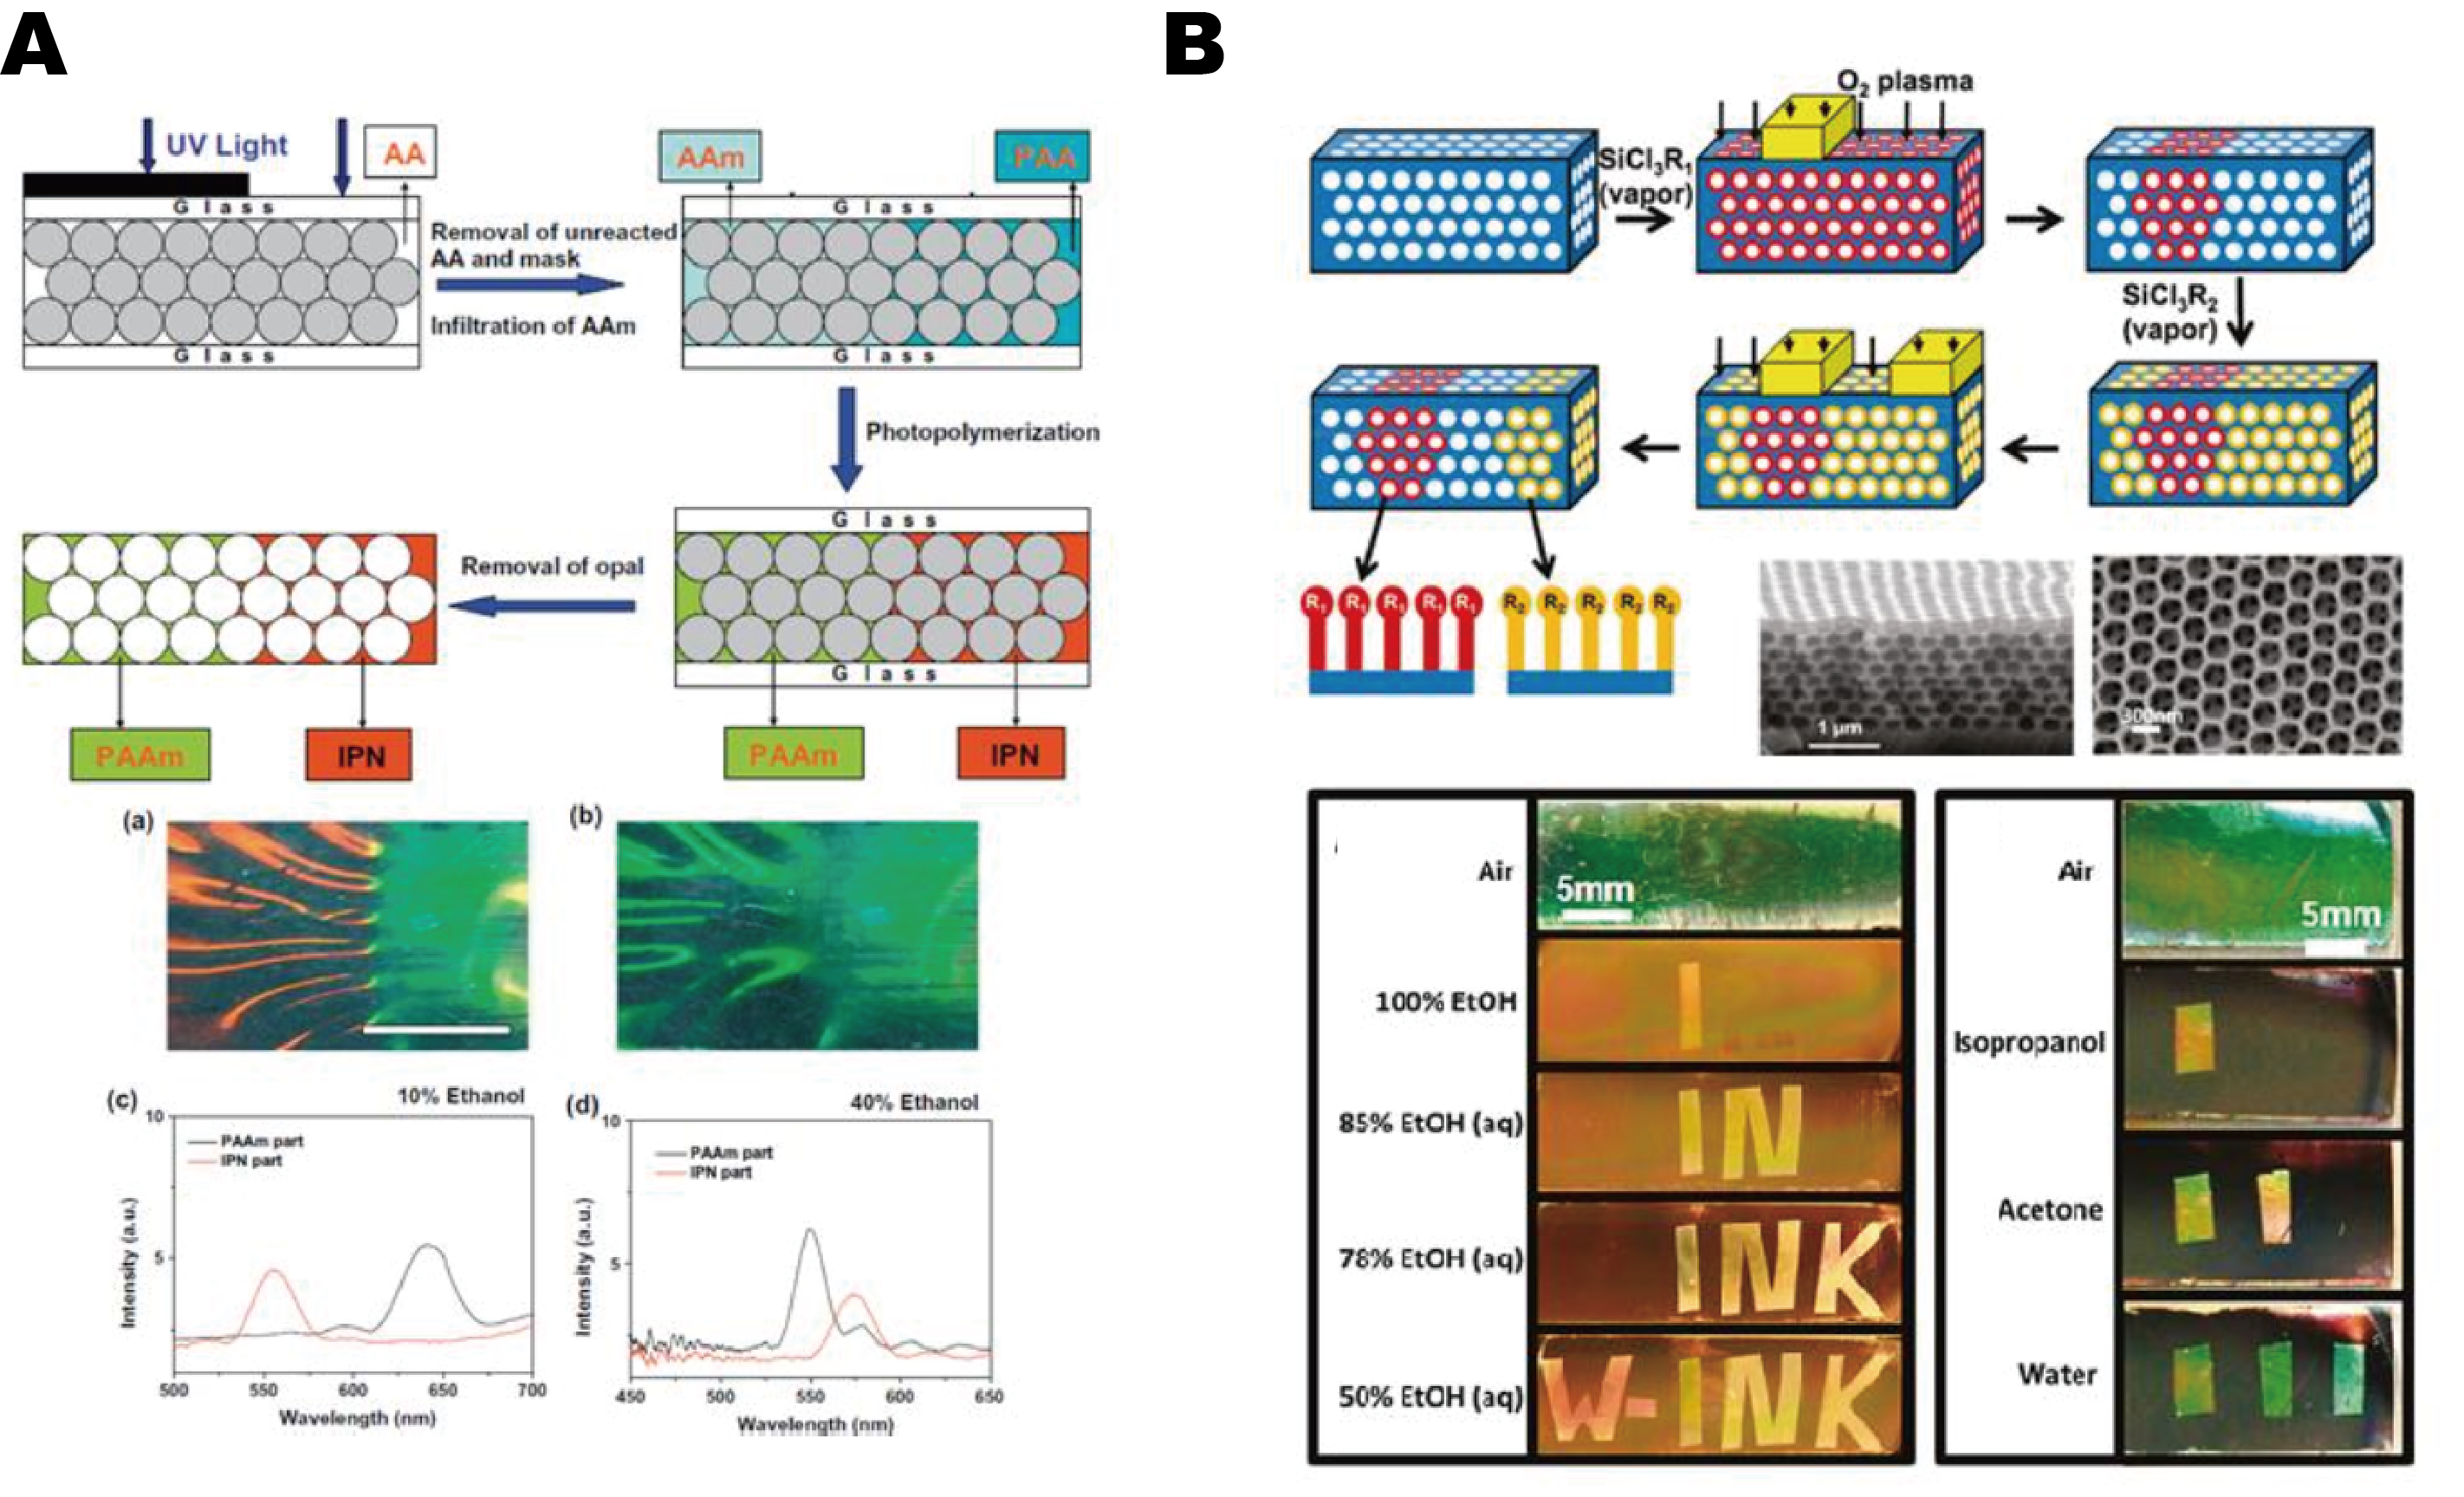
\includegraphics[width=0.9\linewidth]{figures/inverse_opal_pattern.png}
	\caption{反蛋白石光子的晶体层次化技术。A.利用拓扑聚合法的反蛋白石光子晶体二元图案\cite{Wang2011Tuning};B.利用反应等离子化学修饰的反蛋白石光子晶体亲疏水性图案\cite{Burgess2012Encoding}}
	\label{fig:inverse_opal_pattern}
\end{figure}

此外,还可以通过可控表面修饰的方法来进行反蛋白石光子晶体图案化。
Aizenberg等利用二氧化硅表面在反应等离子气氛中的表面亲疏水变化,
制备了具有不同亲疏水性图案化的二氧化硅反蛋白石光子晶体材料\cite{Burgess2012Encoding}。
由于采用定向等离子束及掩膜技术,这种方法能够制备很高精度的图案。
同时,由于反蛋白石光子晶体的孔道瓶颈,使得不同的溶剂在光子晶体中具有不同的通透性,改变对应图案部分的光子禁带,从而使这种材料能够对不同表面张力的溶剂产生图案化响应。

\section{本文的主要研究内容与贡献}
\label{sec:contribute}

\subsection{本文研究的目标与意义}
本课题的主要研究目标为构建一系列基于化学反应的光子晶体多功能材料。基于化学反应的光子晶体材料不仅可以作为多种特定反应底物的响应材料,同时赋予了光子晶体相当大的拓展性。除了各向同性的光子晶体材料之外,本文也研究了平面及球形光子晶体材料的层次化修饰方法,并与化学反应相结合,使这种光子晶体材料能够作为一种具有普适性的功能平台。

\subsection{本论文的结构}
\label{subsec:chapters}

本文主要研究了基于化学反应的多功能化光子晶体材料。各章节中按照递进的顺序分别介绍了各种不同的光子晶体材料的制备、表征及功能化等相关问题。

第~\ref{ch:synth_PhC}章主要介绍了本文中所使用的光子晶体材料的制备方法,包括溶剂挥发诱导的垂直沉积法、逐层堆积法以及微流控液滴制备法生长的光子晶体材料。

第~\ref{ch:maleimide}章介绍了一种基于马来酰亚胺巯基的活性光子晶体材料,并利用马来酰亚胺-巯基的反应,对乙酰胆碱酯酶的活性进行了传感,并在此基础上进行了诸如酶动力活性及抑制剂的筛选等应用。

第~\ref{ch:photoactive}章介绍了一种利用光敏聚合物进行的平面三维反蛋白石光子晶体材料的功能化与图案化方法。利用硝基藜芦醇氨基甲酸酯(NVOC)保护基在紫外光照条件下的可控脱保护及进一步的后续修饰,发展了一种可拓展的平面反蛋白石光子晶体材料。并在此基础上展示了光子晶体梯度禁带及响应性图案等应用,制备了具有二维尺度上的化学复杂性的光子晶体材料。

第~\ref{ch:etch-reaction}章介绍了在光子晶体微球上的层次化方法。通过可控的SiO\text{$_2$}刻蚀-反应,成功发展了一种具有三维化学复杂性的光子晶体微球材料。同时,基于不同的功能化方法,展示了其在亲疏水性梯度、正交化学反应平台、酶级联反应等方面的应用。

第~\ref{ch:conclusion}章总结了本文的工作与基于化学反应的三维光子晶体功能化材料的优势。同时对该种材料的未来发展提出了展望。


